\documentclass[a4paper,12pt,oneside]{book}

%-------------------------------Start of the Preable------------------------------------------------
\usepackage[english]{babel}
\usepackage[utf8]{inputenc}
\usepackage{blindtext}
%packagr for hyperlinks
\usepackage{hyperref}
\hypersetup{
    colorlinks=true,
    linkcolor=blue,
    filecolor=magenta,      
    urlcolor=cyan,
}

\urlstyle{same}
%use of package fancy header
\usepackage{fancyhdr}
\usepackage{float}
\usepackage{subfig}
\setlength\headheight{26pt}
\fancyhf{}
%\rhead{
\includegraphics[width=1cm]{logo}}
\lhead{\rightmark}
\rhead{
\includegraphics[width=1cm]{logo}}
\fancyfoot[RE, RO]{\thepage}
\fancyfoot[CE, CO]{\href{http://www.e-yantra.org}{www.e-yantra.org}}

\pagestyle{fancy}

%use of package for section title formatting
\usepackage{titlesec}
\titleformat{\chapter}
  {\Large\bfseries} % format
  {}                % label
  {0pt}             % sep
  {\huge}           % before-code
 
%use of package tcolorbox for colorful textbox
\usepackage[most]{tcolorbox}
\tcbset{colback=cyan!5!white,colframe=cyan!75!black,halign title = flush center}

\newtcolorbox{mybox}[1]{colback=cyan!5!white,
colframe=cyan!75!black,fonttitle=\bfseries,
title=\textbf{\Large{#1}}}

%use of package marginnote for notes in margin
\usepackage{marginnote}

%use of packgage watermark for pages
%\usepackage{draftwatermark}
%\SetWatermarkText{
\includegraphics{logo}}
\usepackage[scale=2,opacity=0.1,angle=0]{background}
\backgroundsetup{
contents={
\includegraphics{logo}}
}

%use of newcommand for keywords color
\usepackage{xcolor}
\newcommand{\keyword}[1]{\textcolor{red}{\textbf{#1}}}

%package for inserting pictures
\usepackage{graphicx}

%package for highlighting
\usepackage{color,soul}

%new command for table
\newcommand{\head}[1]{\textnormal{\textbf{#1}}}


%----------------------End of the Preamble---------------------------------------


\begin{document}

%---------------------Title Page------------------------------------------------
\begin{titlepage}
	\raggedright
	{\Large eYSIP2016\\[1cm]}
	{\Large\scshape GREENHOUSE POWER MONITORING AND APPLIANCE CONTROL \\[.1in]}
	
	\vfill
	
	{\underline{\large{Interns:}}} \\
	\begin{quote}
		\large{Avilash Mohanty}
		
		\large{Email: avilashmohanty1920@gmail.com}		
		
		\large{Mobile: 9560372680}
	\end{quote}
	
	
	
	\begin{quote}
		\large{Abhishek Acharya}
		
		\large{Email: abhi11796acharaya@gmail.com}	
		
		\large{Mobile: 8014692750}
	\end{quote}
	
	
	\vspace{0.5cm}
	
	{\underline{\textbf{Mentors:}}} \\
	\begin{quote}
		\large{Saurav Shandilya}\\
		\large{Vishwanathan Iyer}\\
		\large{Parin Chheda}\\
		\large{Email: @gmail.com}\\
		\large{Email: @gmail.com}\\
		\large{Email: @gmail.com}\\
		
	\end{quote}
	
	
	
	\begin{flushright}
		{\large Duration of Internship: $ 10/06/2016-24/07/2016 $ \\}
		
	\end{flushright}
	{\itshape 2016, e-Yantra Publication}
	
	
	
\end{titlepage}
%-------------------------------------------------------------------------------

\tableofcontents
%-------------------------------------------------------------------------------
\chapter[GREENHOUSE POWER MONITORING AND APPLIANCE CONTROL]{Greenhouse Power Monitoring and appliance control }
\section{Abstract}
\hspace{7mm}This project aims at developing a web portal with the help of which various aspects of the greenhouse such as ON/OFF Switching,Scheduled ON/OFF ,Graphical Visualization of Real-Time Monitored data collected from "Smart Switchboard/plug" which can provide support upto 3 devices, logging and storage of past data and graphical visualizaton .\\

This web based GUI allows remote access and monitoring capabilities to the user .\\

\newpage

\section{Completion status}
\begin{itemize}
	\item{Tasks Accomplished}
	\setlength\itemsep{0.2cm}
	\begin{enumerate}
		\item{Literature survey of existing Real time Web Monitoring sites. }    
		\item{Developing a Circuit to measure Current,Voltage,Phase,Frequency.}
		\item{Research and finalisation on Micro-controller board and Softwares to be used.}
		\item{Measurement of Current,Phase,Frequency,Voltage.}
		\item{Establishing a connection between server and micro-controller.}
		\item{Logging of Real time data in database.}
		\item{Creating Real Time updating Charts.}
		\item{Graphical Visualisation of logged data.}
		\item{Interfaced relay with the micro-controller.}
		\item{Created a page to control the connected devices.}
		\item{Added Scheduling feature. }
		\item{Added 3 device Support for monitoring and controlling.}
		\item{Created a feedback system to compare real-device status and system's  data.}
		\item{Created a GUI on cool term to configure the 'Smart Switchboard/Plug'.}
		\item{Code Documentation and Project Report.}
	\end{enumerate}
	\item{Incomplete Tasks}
	\begin{enumerate}
		\item{Responsive web design. }
	\end{enumerate}
	\par Front-end can be improved and made responsive by using bootstrap.   
\end{itemize}

\newpage
\section{Hardware parts}
\begin{enumerate}
  \item \textbf{List of hardware used:-}\\
  
		 \begin{tabular}{|l|c|c|}
		 	\hline
		 	\textbf{Name of hardware} & \textbf{Specification} & \textbf{Quantity} \\ \hline
		 	Electrical Switch Board& 2-Plug and 1 Bulb Holder & 1\\ \hline
		 	Potential Transformer& 230V-9V 100mA &1 \\ \hline
		 	Hall Effect Sensor Module& ACS712 (30A) &3\\ \hline
		 	Bulb& 100W & 1\\ \hline
		 	& TI's CC3200-LAUNCHXL&\\
		 	CC3200-LAUNCHPAD&\textit{(With CC3200-HZ on } &1 \\
		 	&\textit{ chip wifi microcontroller)} &\\\hline
		 	Soldring Iron& 220V, 40W &1 \\ \hline
		 	Soldring Wire& 50gm & 1 \\ \hline
		 	Jumper Wires& Female to Female & \\\cline{2-3}
		 	&Male to Female& \\\hline
		 	4-Channel Relay Board& 230V AC (10Amp)& 1\\ \hline
		 	Measurement Board& & \\ 
		 	\textit{(Designed \& Developed } & MBV1.1 & 1 \\
		 	\textit{ \hspace{1cm}By Eyantra) } & & \\ \hline
		 \end{tabular}
		 \vspace{1cm}
	\item \textbf{Details of hardware used:-}
	\begin{itemize}
		  \item Electrical Switch Board  \href{http://www.amazon.in}{Vendor link} 
		  \item Potential Transformer \href{http://www.amazon.in/Input-Output-EI-41x20-5-Power-Transformer/dp/B01I1ZMGKW/ref=sr_1_5?ie=UTF8&qid=1469263889&sr=8-5&keywords=9v+transformer}{Vendor link}
		  \item Hall Effect Sensor Module \href[page=5]{./datasheet/ACS712-Datasheet.pdf}{Datasheet, page 5}, \href{http://www.amazon.in/Current-Sensor-Module-ACS712-model/dp/B00NU8XD80?tag=googinhydr18418-21&tag=googinkenshoo-21&ascsubtag=8a34ff38-5122-429d-8260-7633d5ca1fcf}{Vendor link},
		  \item Bulb  \href{http://www.amazon.in}{Vendor link}
		  \item CC3200 LAUNCHPAD \href[page=5]{./datasheet/cc3200 complete datasheet.pdf}{Datasheet, page 5}, 		\href{https://www.fabtolab.com/boards/TI}{Vendor link}
		  \item Jumper Wires  \href{https://www.fabtolab.com}{Vendor link}
		  \item 4-Channel Relay Board \href[page=5]{./datasheet/relay.pdf}{Datasheet, page 5}, \href{https://www.fabtolab.com}{Vendor link}
		  \item Measurement Board \autoref{100}
	\end{itemize}
	\newpage
  \item \textbf{Connection diagram:-}
  \begin{figure}[h]
  	\includegraphics[width=390px]{connection}
  \end{figure}
  \\\textbf{HERE:-} 
   \begin{itemize}
   	\item A1:  current sensor input pin 1
   	\item A2:  current sensor input pin 2
   	\item A3:  current sensor input pin 3
   	\item V1:  transformer output pin
   	\item C1:  current1 signal out pin 
   	\item C2:  current2 signal out pin
   	\item V1:  voltage signal out pin
   	\item F1:  frequency signal out pin
   	\item PH1:  phase 1 signal out pin
   	\item PH2:  phase 2 signal out pin
   \end{itemize}
\end{enumerate}

\newpage
\section{Software used}
\begin{enumerate}
	\item\textbf{ Code Composer Studio} \\
  -- Detail of software: version 6.1.3.00033, \href{http://www.ti.com}{download link}\\
  -- Installation steps:
  \begin{itemize}
  	\item click on the rar file named $"CCS6.1.3.00033_win32"$
  	  \begin{figure}[h]
  	  	\hspace{2cm}
  	 	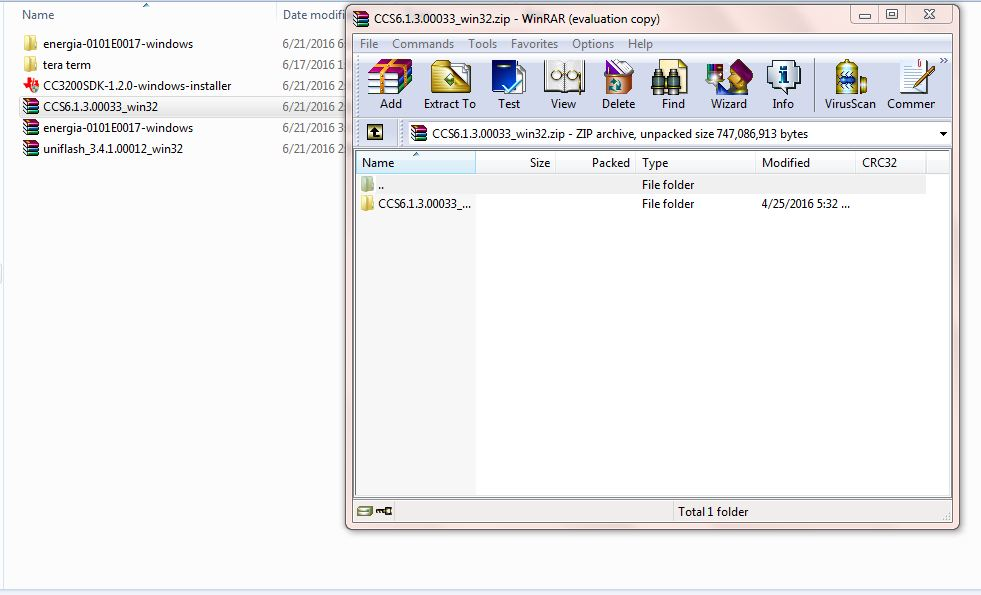
\includegraphics[width=300px]{inst1}
  	 \end{figure}
  	 	 \item Now click on the extracted folder
  	  \begin{figure}[h]
  	  		\hspace{2cm}
  	 	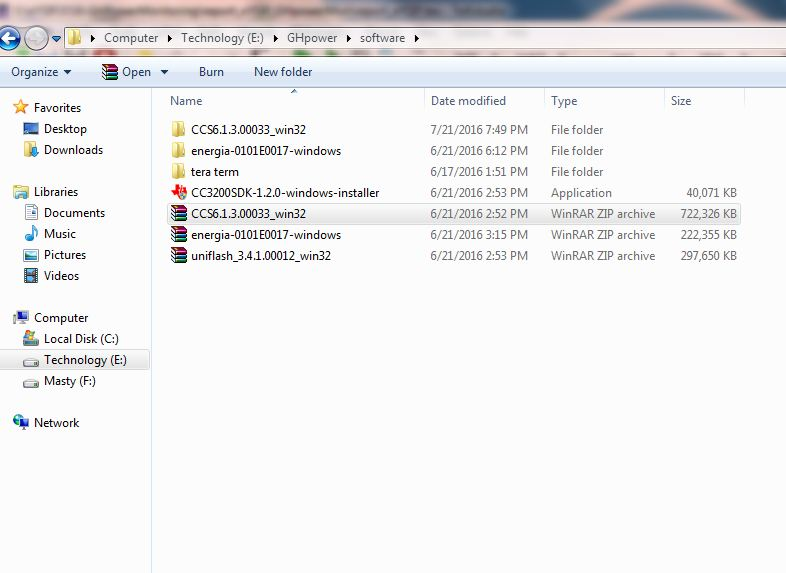
\includegraphics[width=300px]{inst2}
  	 \end{figure}
  	 \newpage
  	 \item click on the .exe setup file
  	 \begin{figure}[h]
  	 		\hspace{2cm}
  	  	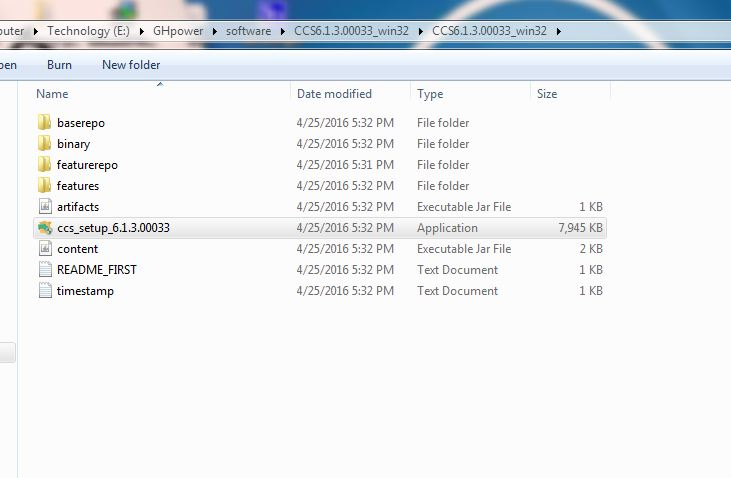
\includegraphics[width=300px]{inst3}
  	 \end{figure}
  	 \item now continue to click on next till complete installation of Code Composer studio
  	 \begin{figure}[h]
  	 		\hspace{2cm}
  	 	
\includegraphics[width=250px]{inst4}
  	  \end{figure} 
  	  \newpage
  	  \item \textbf{Energia}
  	   -- Detail of software: version 6.1.3.00033, \href{http://www.energia.nu}{download link}\\
  	   -- Installation steps:
  	   \begin{itemize}
  	   	\item click on the rar file named $"energia-0101E0017-windows"$
  	   	\begin{figure}[h]
  	   		\hspace{2cm}
  	   		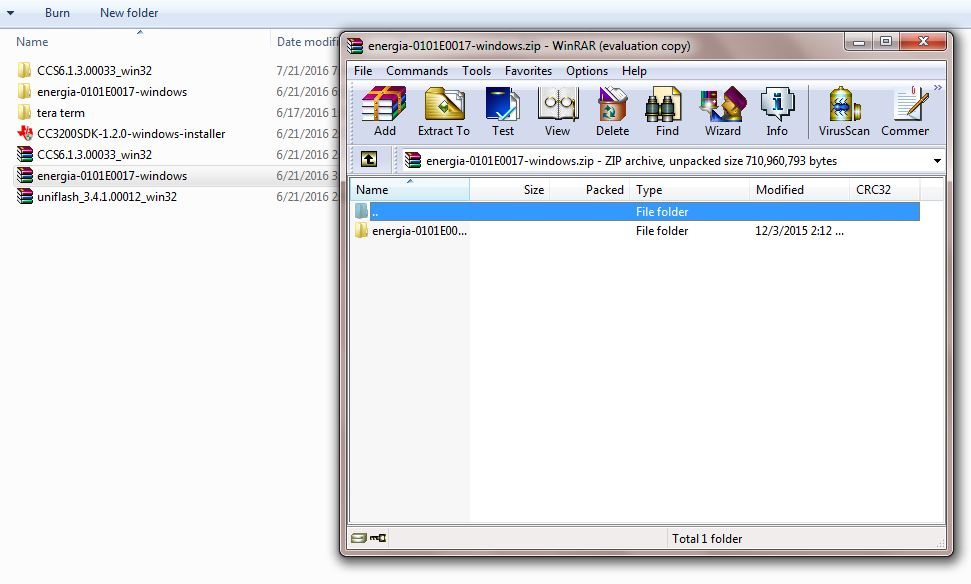
\includegraphics[width=300px]{inst5}
  	   	\end{figure}
  	   \end{itemize}
  	   \item Now click on extracted folder with same name
  	   \begin{figure}[h]
  	   	\hspace{2cm}
  	   	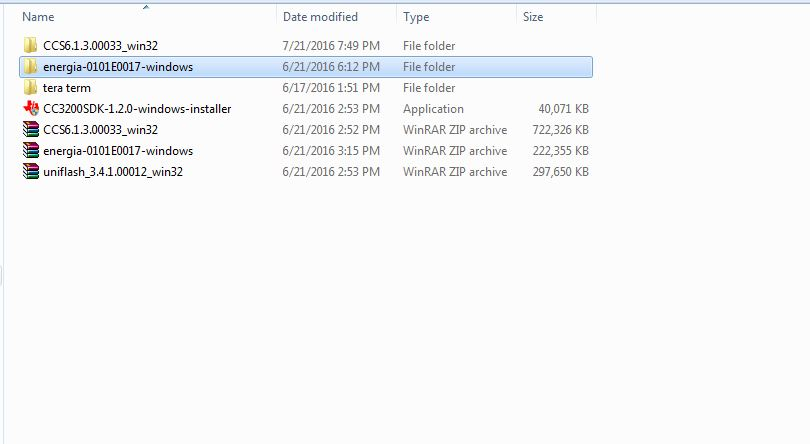
\includegraphics[width=300px]{inst6}
  	   \end{figure}
  	     \newpage
  	   \item click on energia .exe application file
  	   \begin{figure}[h]
  	   	\hspace{2cm}
  	   	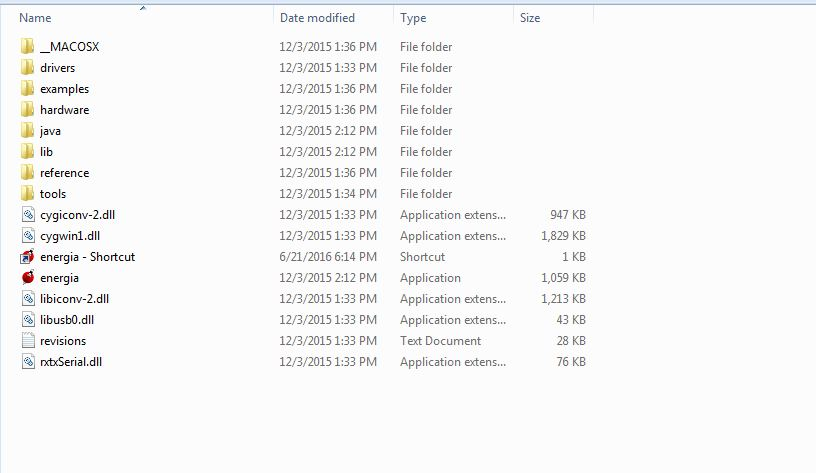
\includegraphics[width=300px]{inst7}
  	   \end{figure}
  	   \item code compile upload and enjoy
  	   \begin{figure}[h]
  	   	\hspace{2cm}
  	   	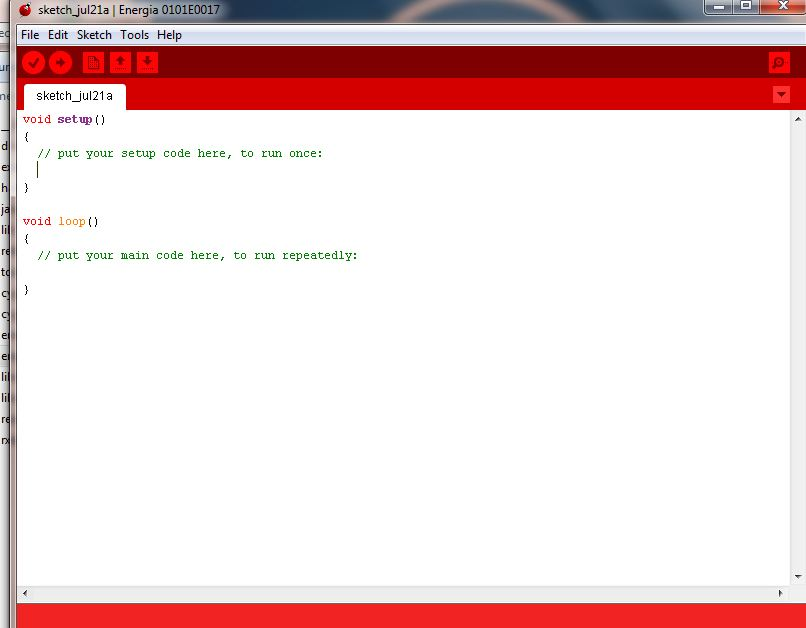
\includegraphics[width=300px]{inst8}
  	   \end{figure}
  \end{itemize}
  \newpage
  	\item\textbf{CCS Uniflash} \\
  	-- Detail of software: version 3.4, \href{http://www.ti.com}{download link}\\
  	-- Installation steps:
    \begin{itemize}
    	\item click on the rar file named $"uniflash_3.4.1.00012_win32"$
    	\begin{figure}[h]
    		\hspace{2cm}
    		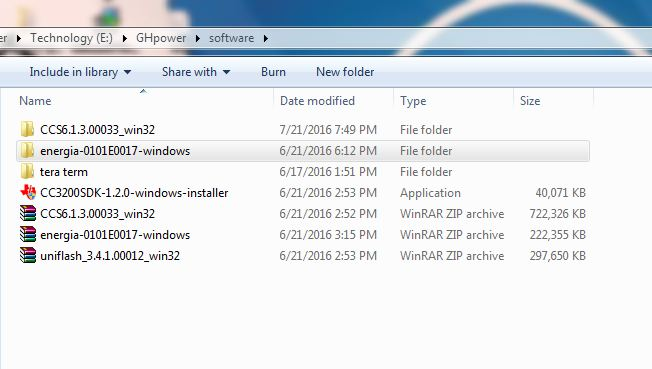
\includegraphics[width=300px]{inst9}
    	\end{figure}
    \item Now click on extracted folder with same name
    \begin{figure}[h]
    	\hspace{2cm}
    	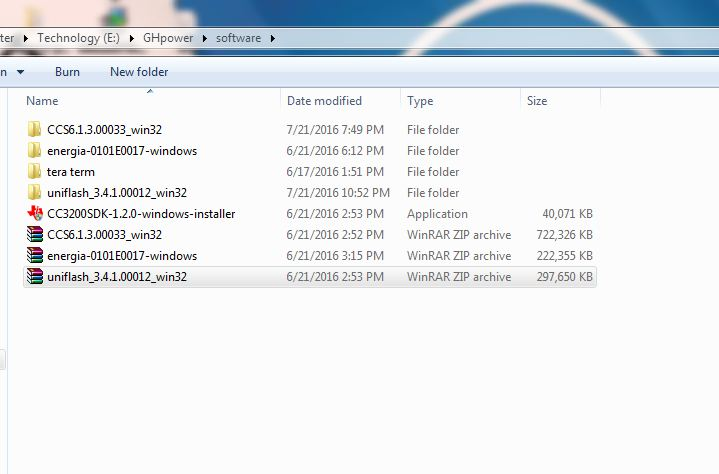
\includegraphics[width=300px]{inst10}
    \end{figure}
    \newpage
    \item click on $uniflash_win.exe$ application file and continue to click on next till installation complete.
    \begin{figure}[h]
    	\hspace{2cm}
    	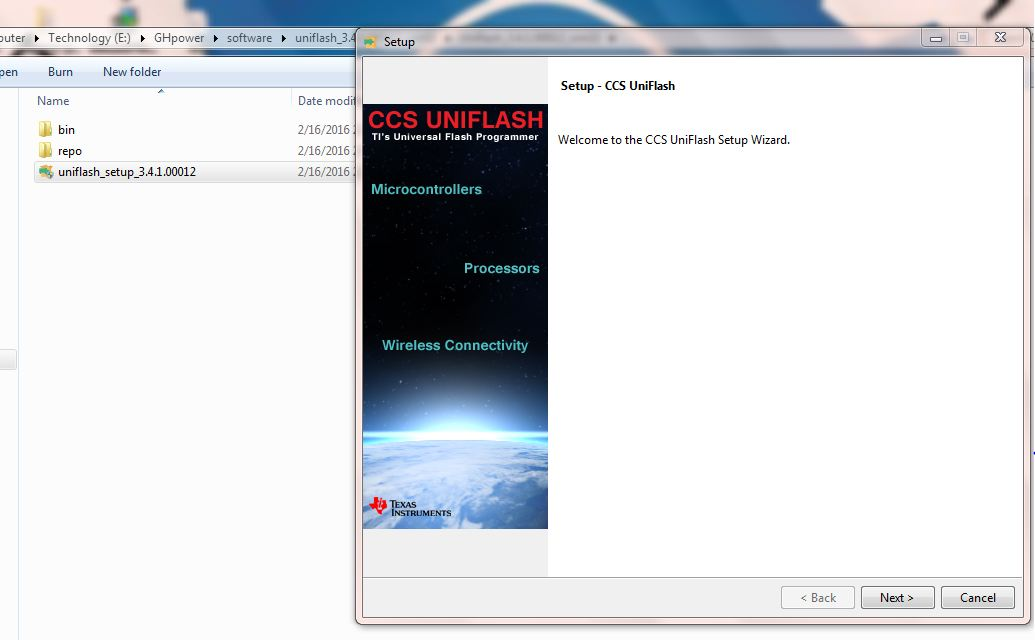
\includegraphics[width=300px]{inst11}
    \end{figure}
    \begin{figure}[h]
    	\hspace{2cm}
    	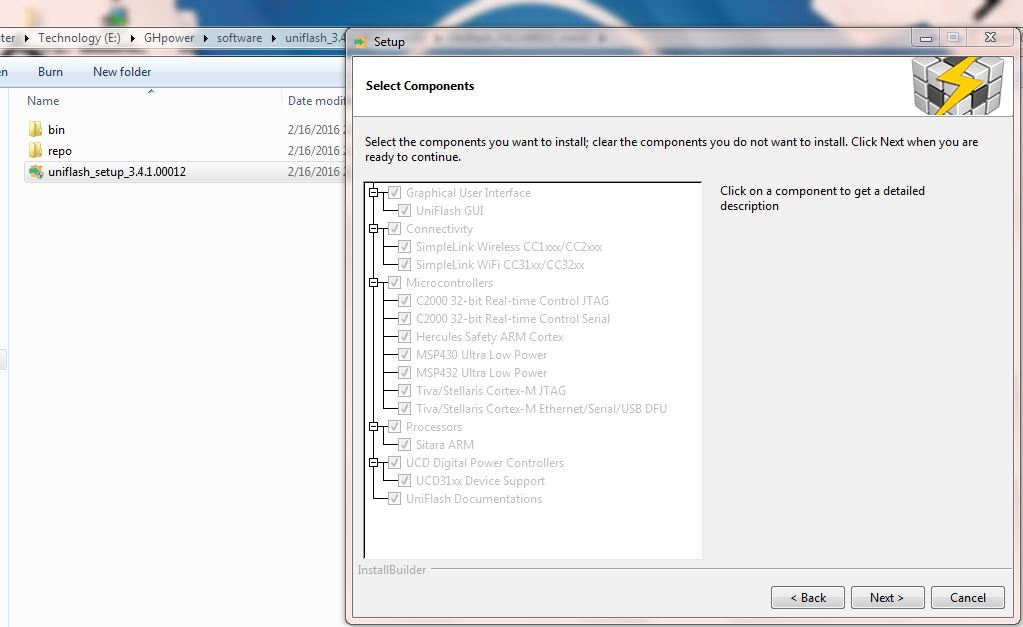
\includegraphics[width=300px]{inst12}
    \end{figure}
    \newpage
     \item open uniflash, select COM port and make a .ccxml file for cc3200 launchpad
     \begin{figure}[h]
     	\hspace{2cm}
     	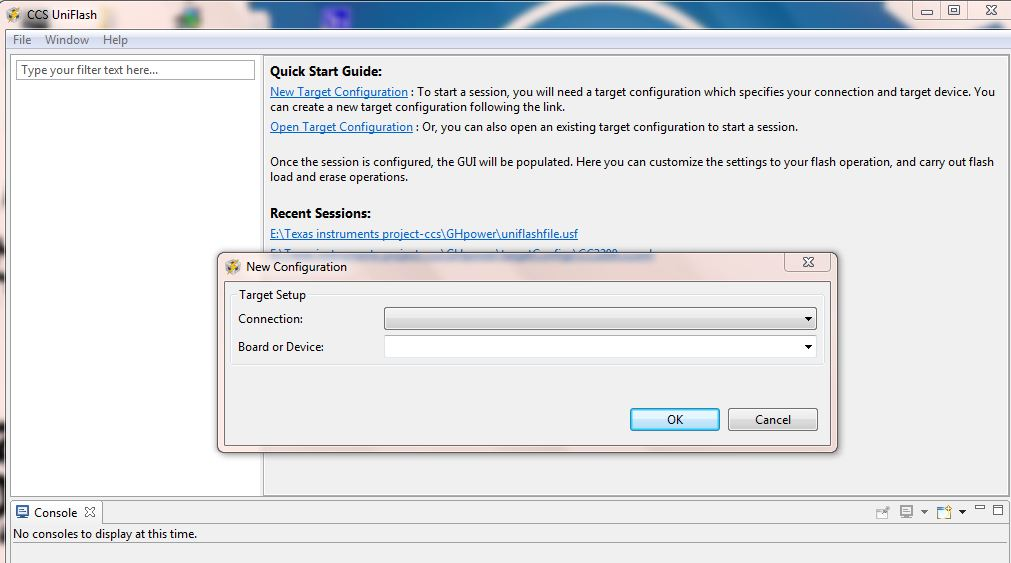
\includegraphics[width=300px]{inst13}
     \end{figure}
\end{itemize}
\newpage
	\item\textbf{ CC3200 SDK from TI} \\
	-- Detail of software: version 1.2.0, \href{http://www.ti.com}{download link}\\
	-- Installation steps:
\begin{itemize}
	 \item click on CC3200SDK.exe application file and install the sdk by clicking next button till installation complete
	 \begin{figure}[h]
	 	\hspace{2cm}
	 	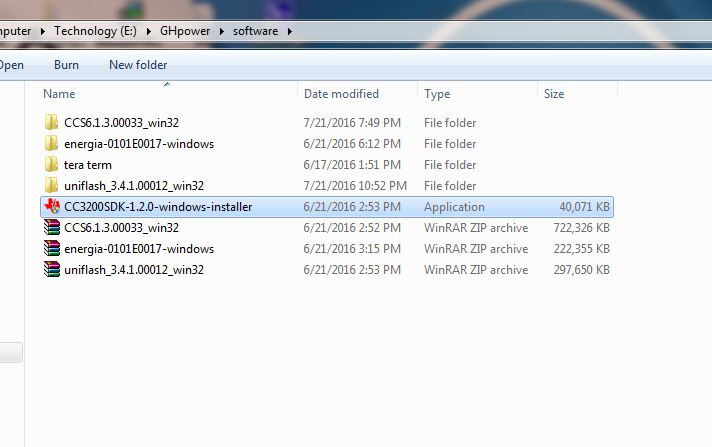
\includegraphics[width=300px]{inst14}
	 \end{figure}
	 \begin{figure}[h]
	 	\hspace{2cm}
	 	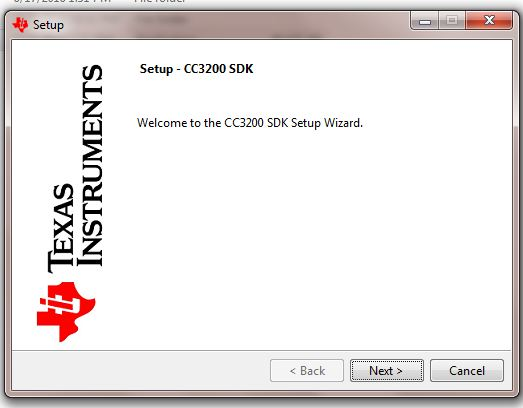
\includegraphics[width=300px]{inst15}
	 \end{figure}
\end{itemize}
\newpage
\item\textbf{ CC3200 service pack} \\
-- Detail of software: version 1.0.0.1.2, \href{http://www.ti.com}{download link}\\
   \textbf{note:- service pack should be compatible with your launchpad version}\\
-- Installation steps:
\begin{itemize}
	\item click on CC3200SDK.exe application file and install the sdk by clicking next button till installation complete
	\begin{figure}[h]
		\hspace{2cm}
		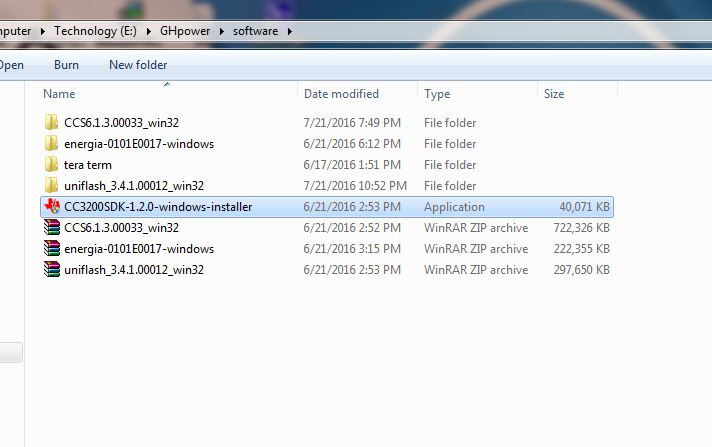
\includegraphics[width=300px]{inst14}
	\end{figure}
	\begin{figure}[h]
		\hspace{2cm}
		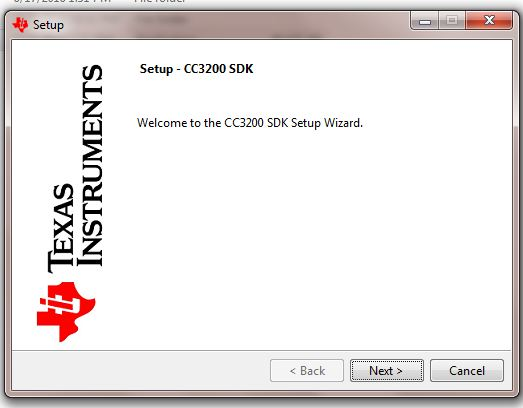
\includegraphics[width=300px]{inst15}
	\end{figure}
\end{itemize}
\newpage
\item\textbf{ Terminal softwares: Coolterm \& Teraterm} \\
-- Detail of software: version 1.4.6, \href{http://www.coolterm.com}{Coolterm}\\
-- Detail of software: version 1.4.6, \href{http://www.coolterm.com}{Teraterm}\\
	\begin{figure}[h]
		\hspace{2cm}
		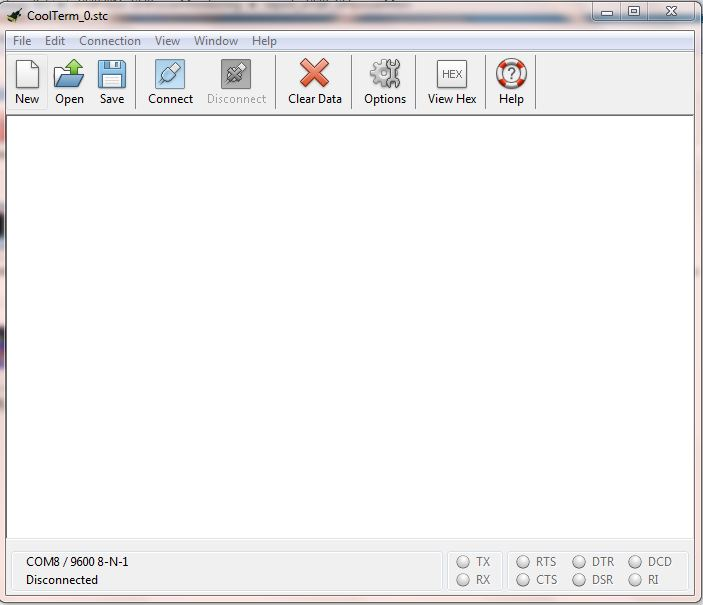
\includegraphics[width=270px]{inst16}
	\end{figure}
	\begin{figure}[h]
		\hspace{2cm}
		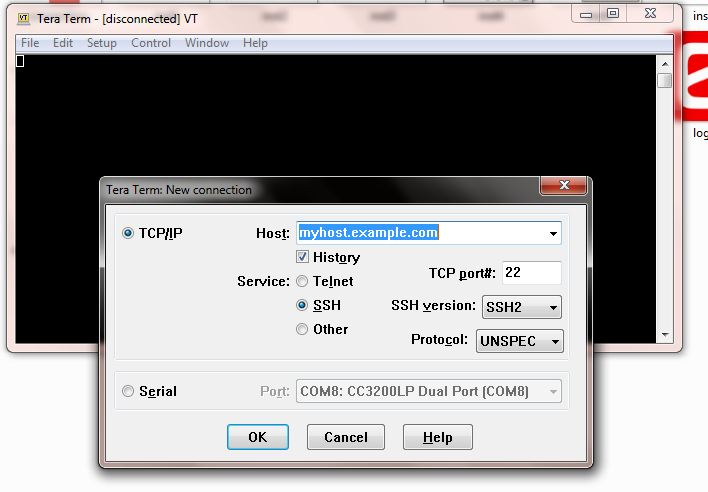
\includegraphics[width=270px]{inst17}
	\end{figure}
	\newpage
					\item Setting up the environment
					\begin{enumerate}
						\item Software used:Windows OS
						\item Version:Windows 10
					\end{enumerate}
					\item Setting up the Server \& Database
					\begin{enumerate}
						\item Software used:XAMPP
						\item Version:XAMPP version 3.2.2
						\item \href{https://www.apachefriends.org/download.html}{XAMPP Download Link}
						\item \href{http://www.wikihow.com/Install-XAMPP-for-Windows}{XAMPP Installation steps.}
						\hspace{20px}
						
						\begin{figure}[H]  \centering
							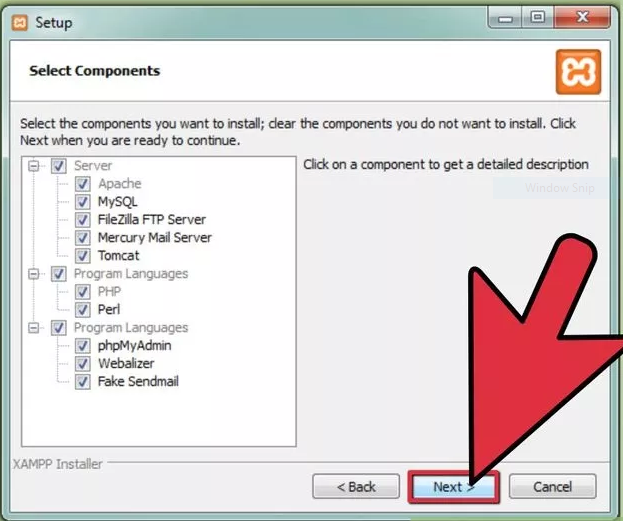
\includegraphics[width=13cm]{xampp1.png}
							\caption{Component Selection}
						\end{figure}
						\begin{figure}[H]  \centering
							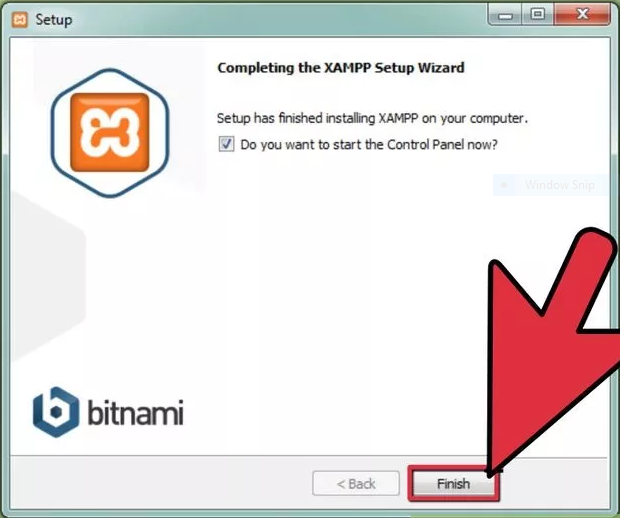
\includegraphics[width=13cm]{xampp12.png}
							\caption{Finish Installation}
						\end{figure}
						\begin{figure}[H]  \centering
							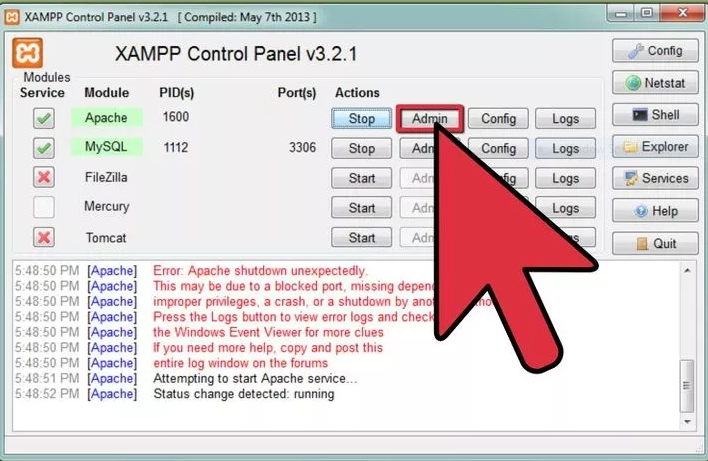
\includegraphics[width=13cm]{xampp3.png}
							\caption{Open XAMPP Control Panel}
						\end{figure}
						\hspace{10px}
						
						\textbf{NOTE: If Server rejects connection requests by microcontroller, follow these steps.}
						
						\begin{figure}[H]  \centering
							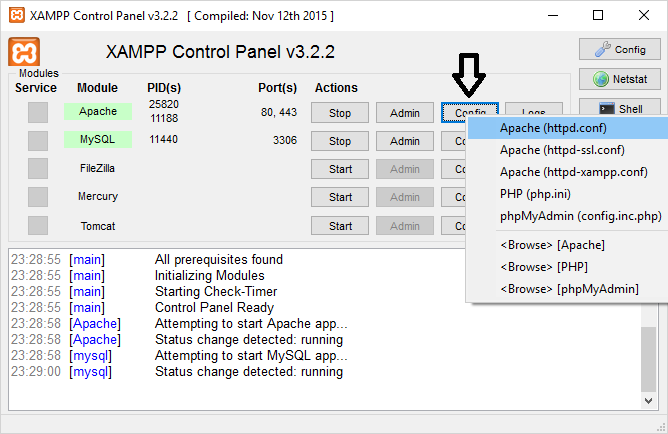
\includegraphics[width=13cm]{httpconf2.png}
							\caption{Open httpd.conf}
						\end{figure}
						
						\item{Open httpd.conf file in configuration setting for Apache Server in XAMPP.}
						\begin{figure}[H]  \centering
							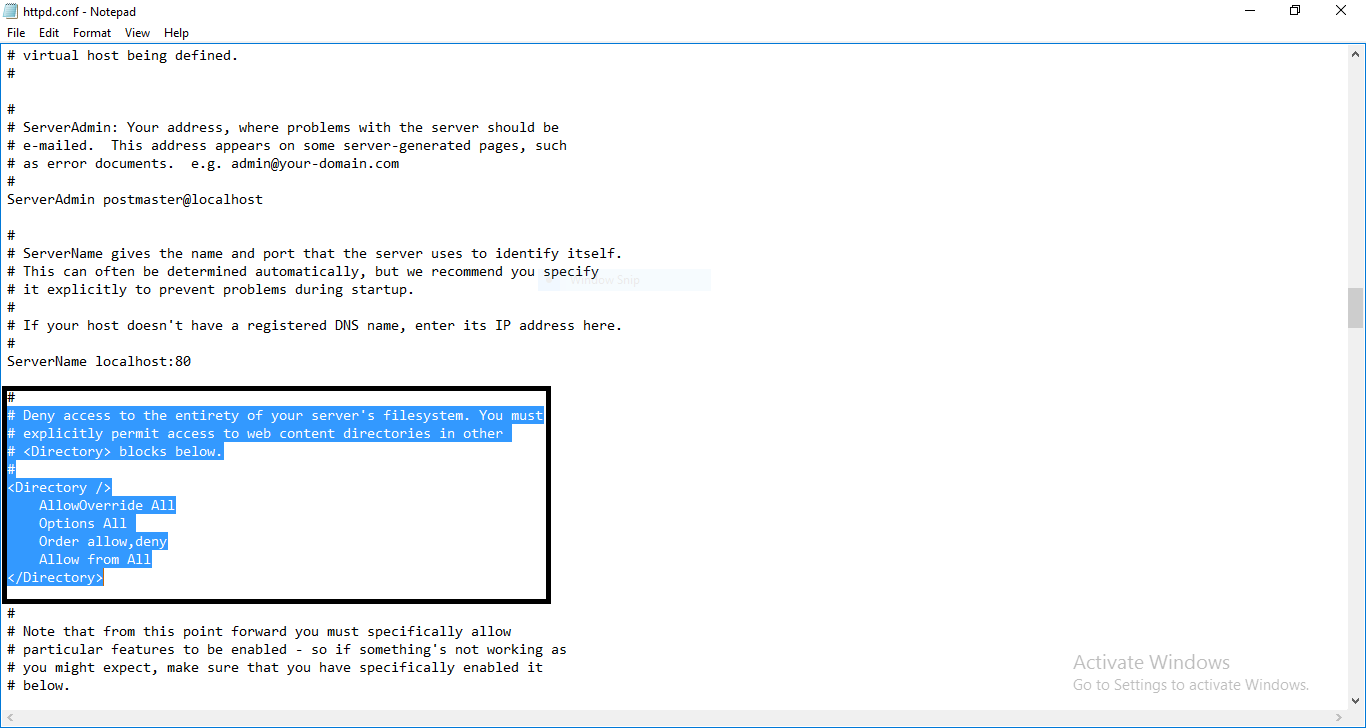
\includegraphics[width=13cm]{override.png}
							\caption{Change httpd.conf}
						\end{figure}
						
						\item{Set\\ $AllowOverride  All$\\
							$Options All$ \\
							$Order allow,deny$\\
							$Allow from All$ }
						
						
					\end{enumerate}
					\item Setting up the Editor
					\begin{enumerate}
						\item Software used:Notepad++ v6.9.2
						\item\href{https://notepad-plus-plus.org/download/v6.9.2.html}{Notepad++ v6.9.2 Download Link}
					\end{enumerate}			
\end{enumerate}

\newpage
\section{Assembly of hardware}
Circuit diagram and Steps of assembly of hardware with pictures for each step
\subsection*{Circuit Diagram}
\begin{figure}[h]
	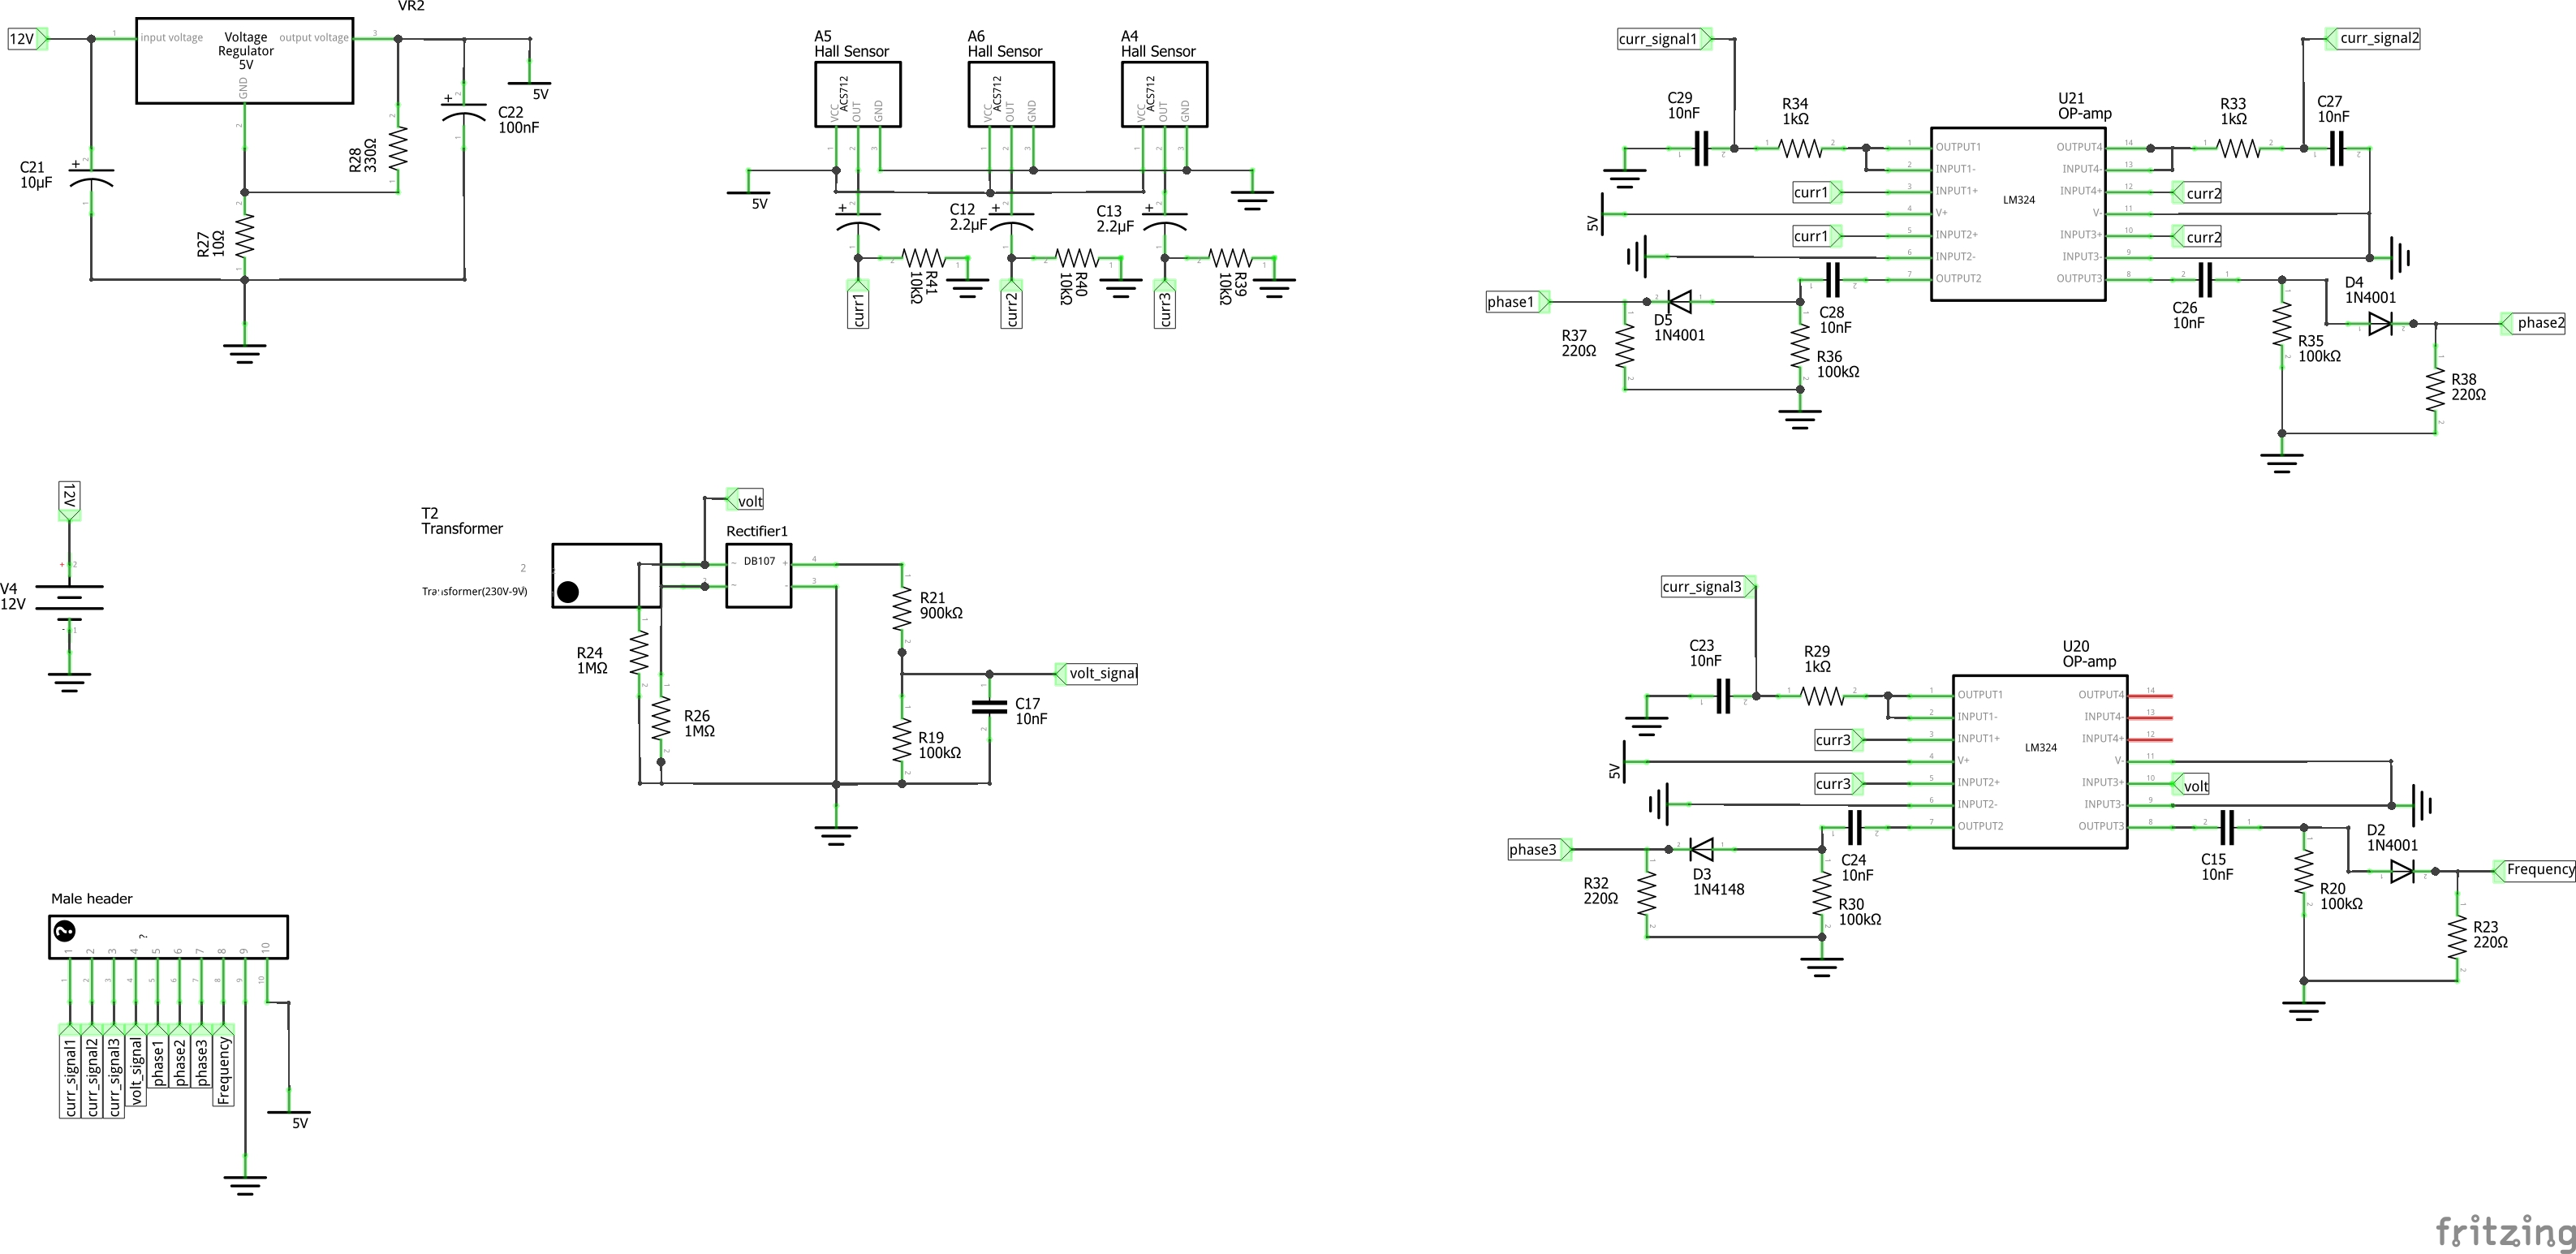
\includegraphics[width=380px,height=380px]{schematic}
\end{figure}
\newpage
\subsection*{Step 1}
Make a basic switch board which has two plug and and one bulb holder mounted on it as 
shown in figure below
\begin{figure}[h]
	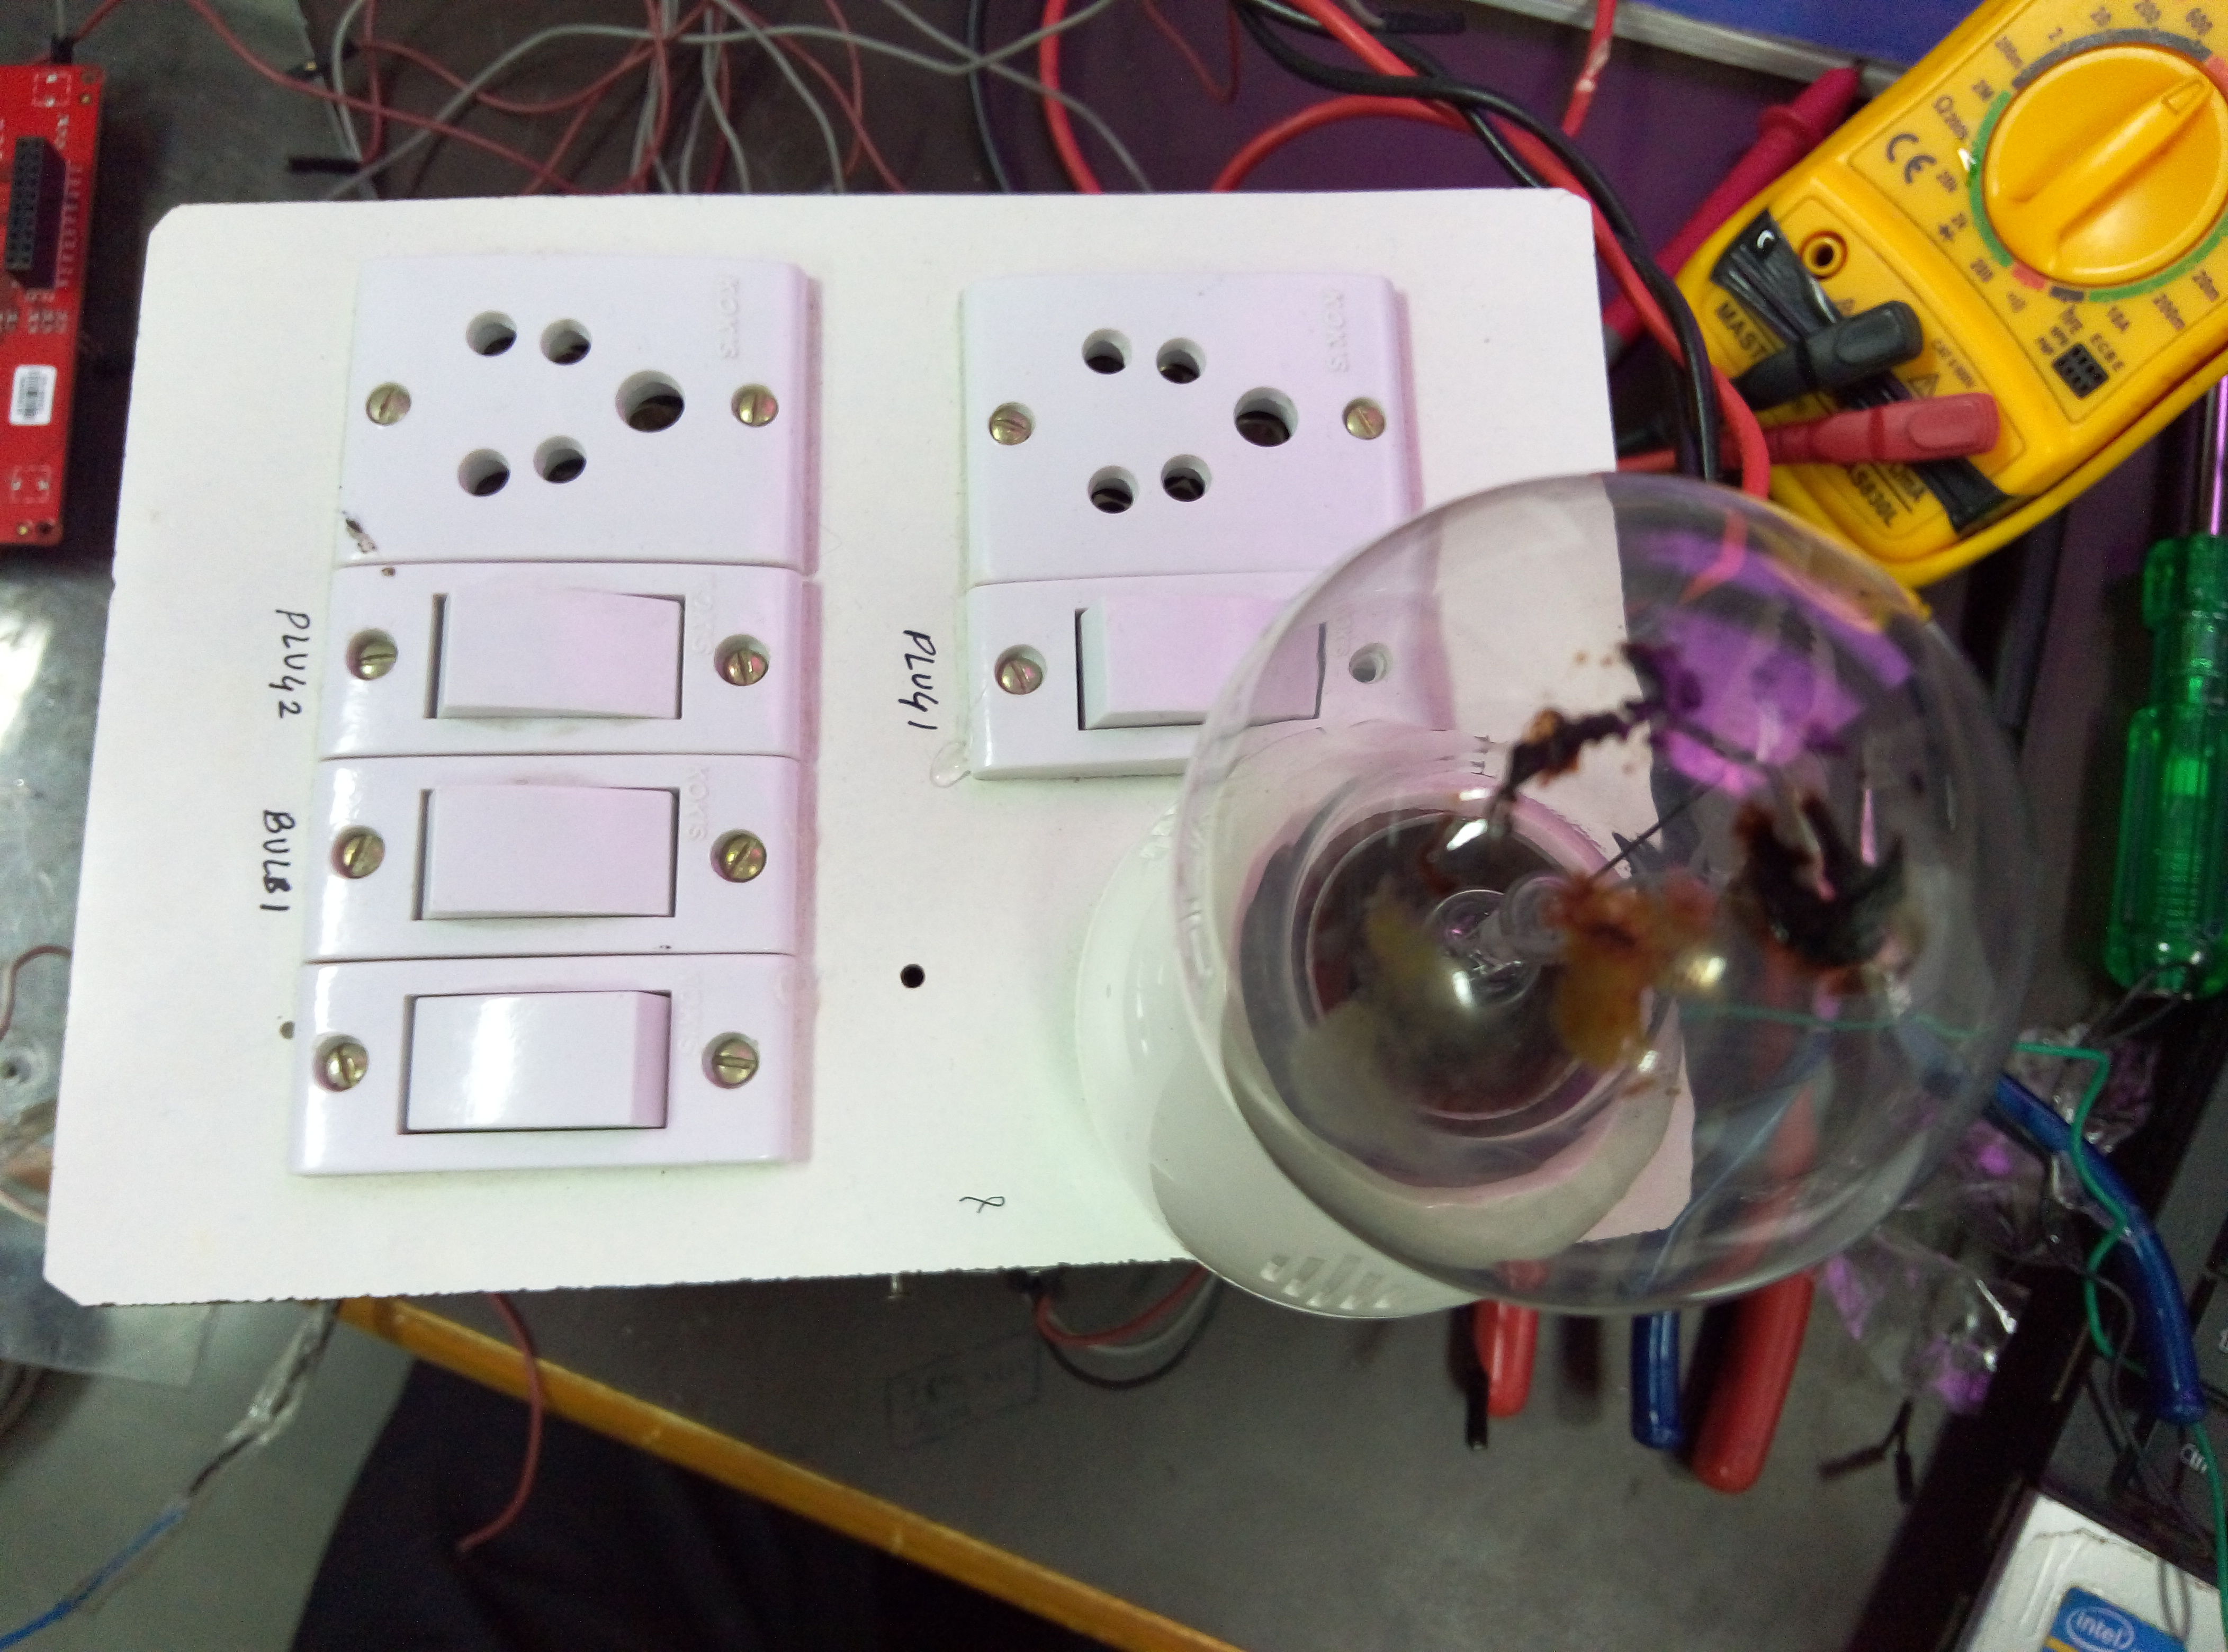
\includegraphics[width=300px]{plug1}
	\includegraphics[width=300px]{plug2}
\end{figure}
\newpage
\subsection*{Step 2}
Now assemble the $"measurement board"$ with the switch board at the location of your convenience. Make sure you have fixed the measurement board permanently with switch board as shown in figure below. 
\begin{figure}[h]
	\includegraphics[width=400px,height=200px]{assem1}
\end{figure}
\subsection*{Step 3}
Now connect and fix relay board with switch board at the location of your convenience as show in figure below
\begin{figure}[h]
	\includegraphics[width=400px,height=200px]{assem2}
\end{figure}
\newpage
\subsection*{Step4}
Now connect the $CC3200-launchpad$ at the male headers 21 and 22. For more detail see board manual \autoref{1}
\begin{figure}[h]
	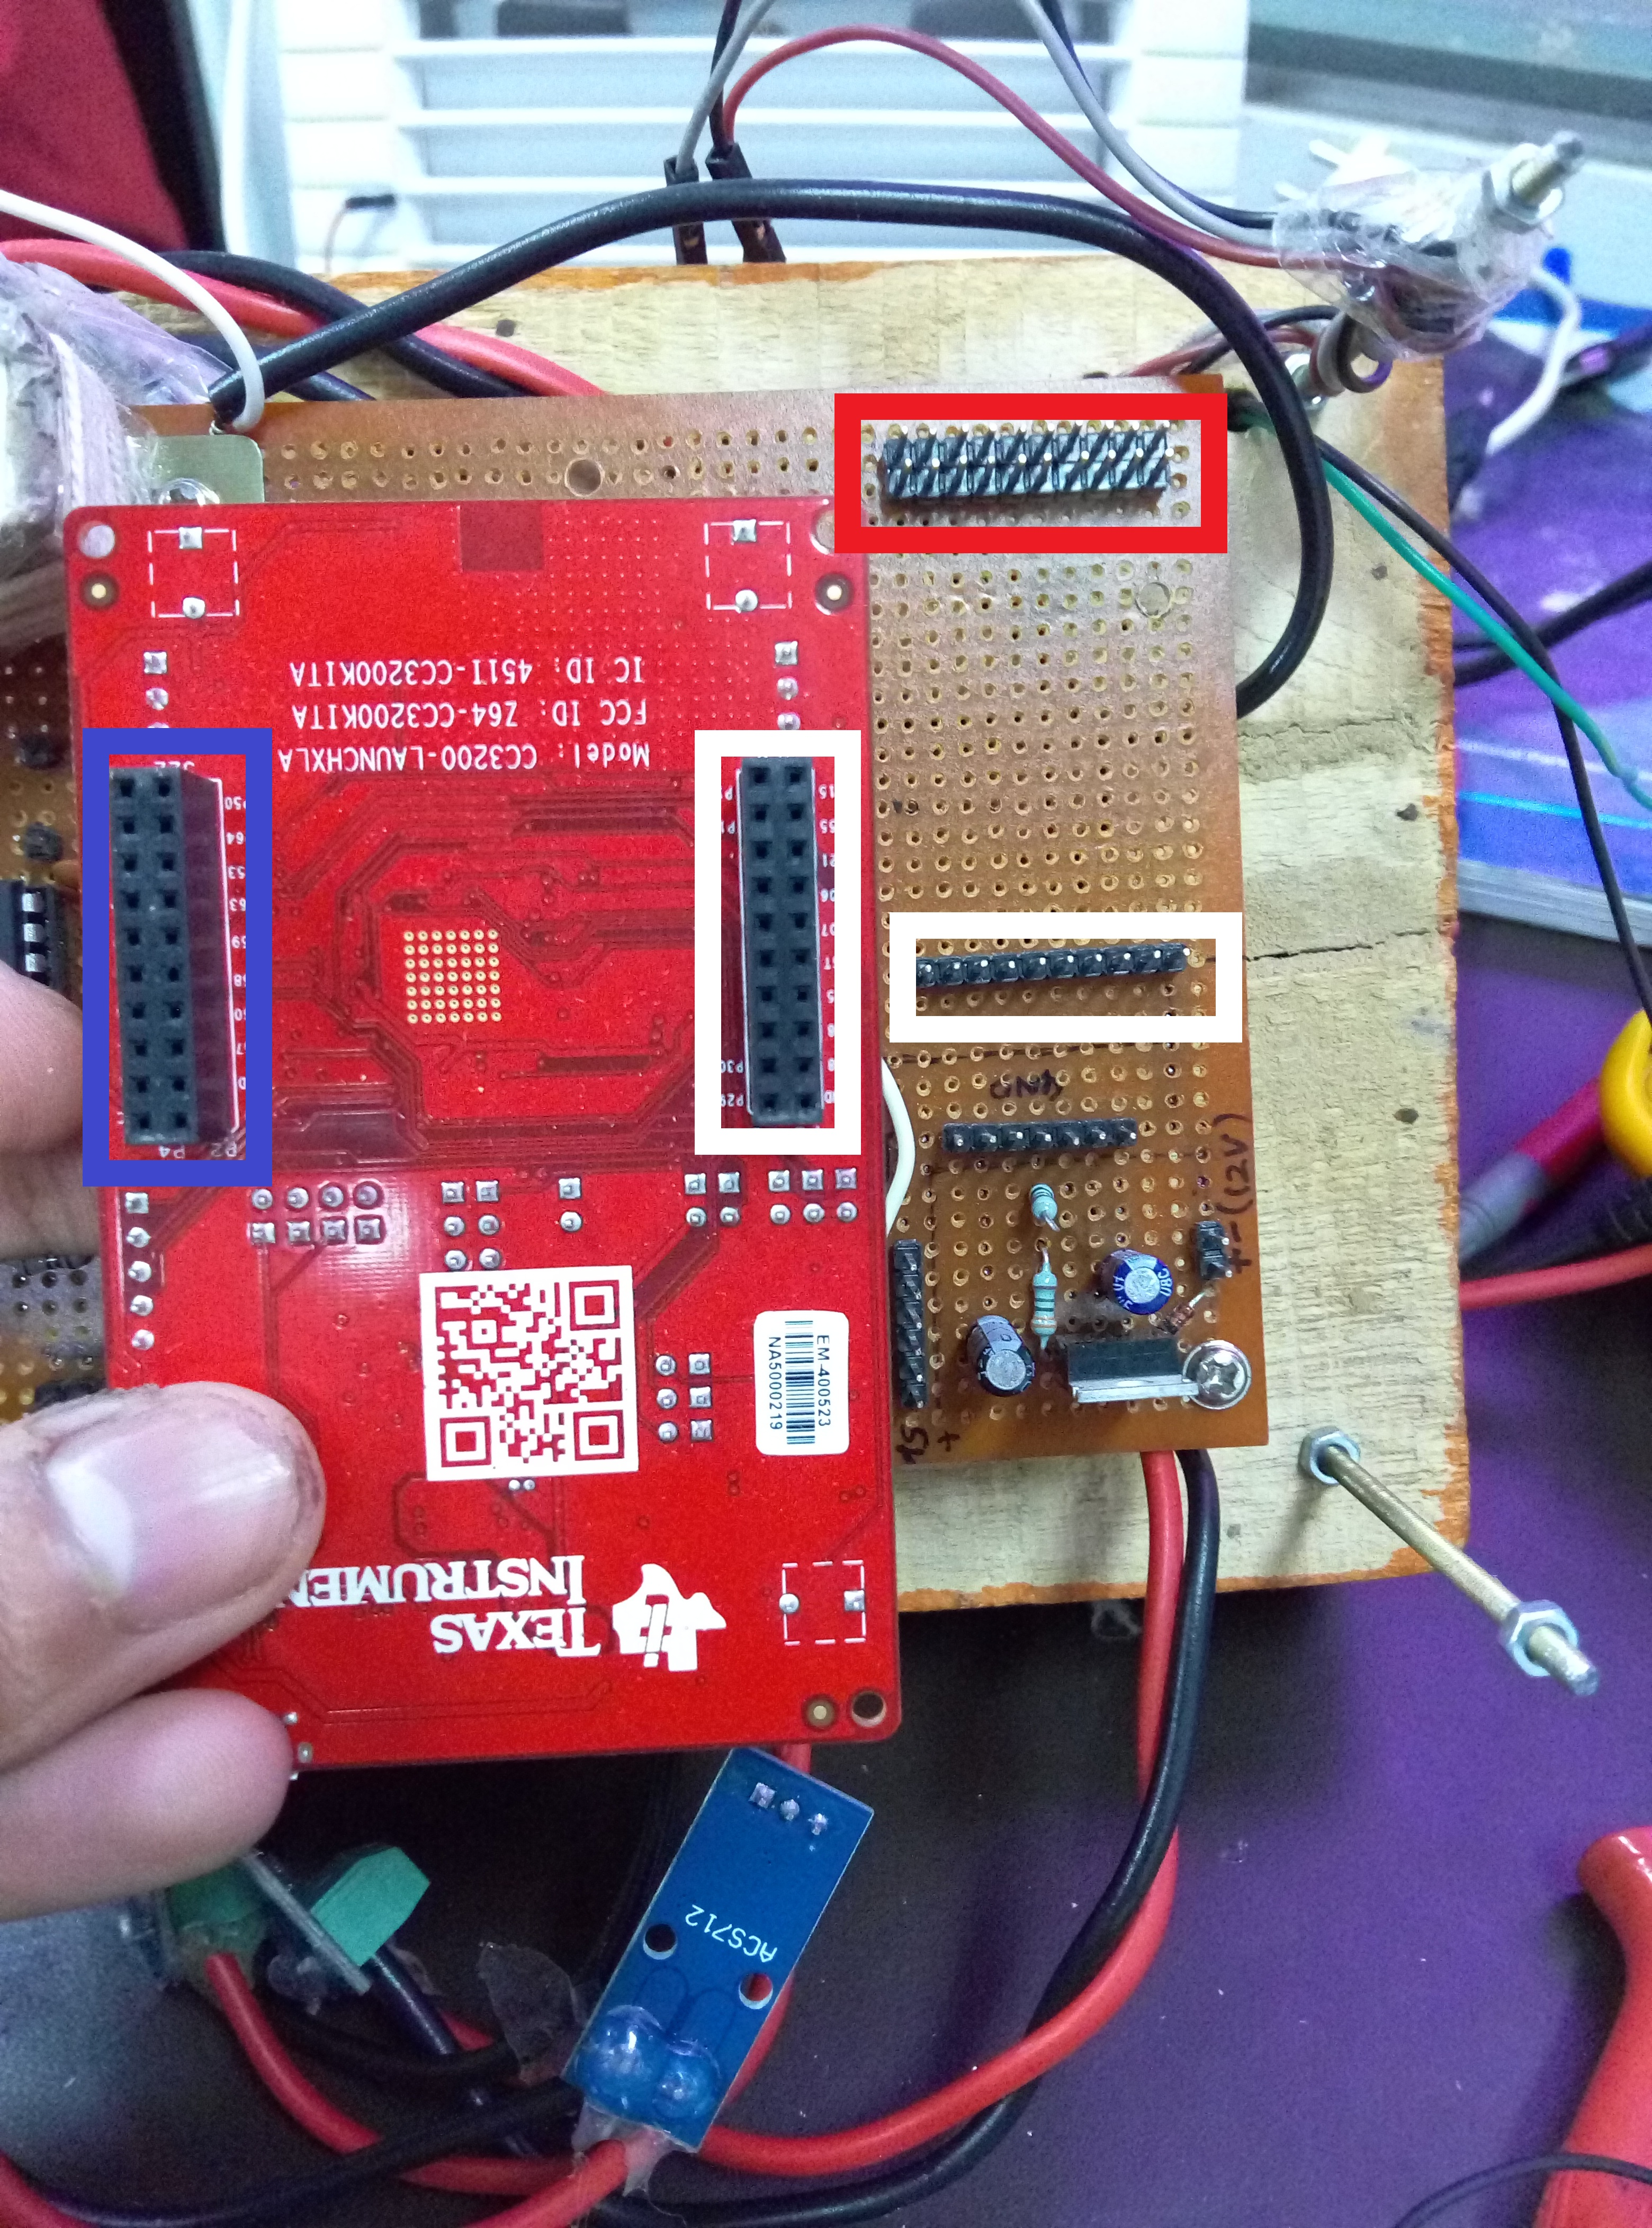
\includegraphics[width=300px,height=200px]{assem3}
\end{figure}
\subsection*{Step5}
Now connect all the three hall sensor at pin number 1,2 and 3 appropriately on measurement board.for more detail see board manual \autoref{1}
\begin{figure}[h]
	\includegraphics[width=300px,height=200px]{assem4}
\end{figure}
\subsection*{Step6}
Now connect $cc3200-launchpad$ and $Transformer$ with measurement board using female jumper as described below:
\begin{itemize}
	\item connect (pin1,pin4),(pin2,pin5) and (pin3,pin7) on the measurement board.
	\item connect pin7 and pin8 with the transformer output jumper.
	\item connect pin9 of measurement board to \textbf{$PIN59$} of cc3200 launchpad.
	\item connect pin17 of measurement board to \textbf{$PIN05$} of cc3200 launchpad.
	\item connect pin10 of measurement board to \textbf{$PIN58$} of cc3200 launchpad.
	\item connect pin12 of measurement board to \textbf{$PIN18$} of cc3200 launchpad.
	\item connect pin14 of measurement board to \textbf{$PIN60$} of cc3200 launchpad.
	\item connect pin15 of measurement board to \textbf{$PIN08$} of cc3200 launchpad.
	\item connect 5V and 3.3V pins of measurement board to $5V$ and $Vcc$ pins of cc3200 launchpad. 
	\item connect "Vcc" and "GND" of relay board with "5V" and "GND" of measurement board.
	\item connect the input pins of relay with $PIN64$, $PIN01$ and $PIN02$
	of CC3200 launchpad.
\end{itemize}
\newpage
\begin{figure}[h]
	\includegraphics[width=350px,height=350px]{assem5}
\end{figure}
for more detail about pin connection see board manual \autoref{1}
\subsection*{Step7}
Now connect some more accessories to improve mechanical design and your \textbf{"Smart switch board"} is ready to use.

\newpage

\section{Software and Code}
\hspace{7mm}\href{https://github.com/eYSIP-2016/eYSIP2016-GHPowerMonitoring}{Github link} for the repository of code.\\


\begin{itemize}
	\setlength\itemsep{0.2cm}
	\item{Sending measured Data to server}
	\begin{itemize}
		
		\begin{figure}[H]
			\centering
			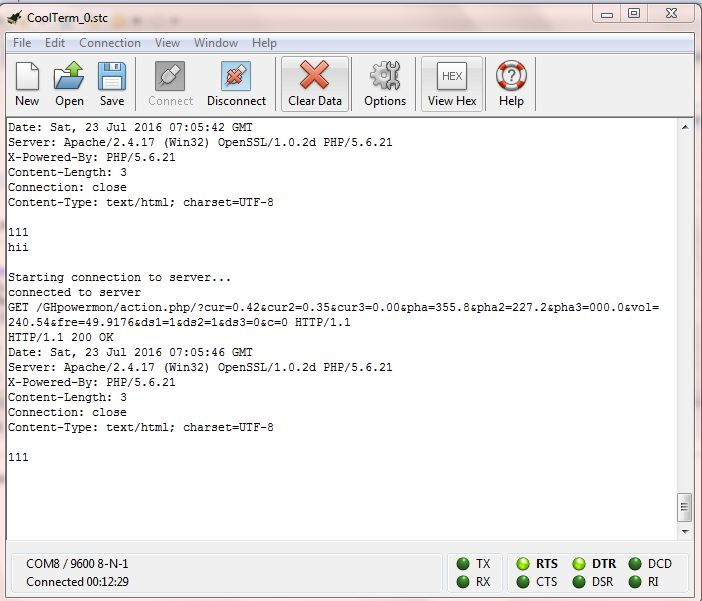
\includegraphics[width=15cm]{coolterm1.jpg}
			\caption{Cool Term - 1}
			\label{29}
		\end{figure}
		
		\item{$action.php$ is the page accessed by the micro-controller, which in turn updates the database according to the data acquired.}
		\item{CC3200 uses queries to POST data and updates current values for devices 1,2,3 using $cur,cur2,cur3$, updates voltage using $vol$, frequency using $fre$,  phase of three devices using $pha,pha2,pha3$.}
	\end{itemize}
	\newpage
	\item{logging the data}
	\begin{itemize}
		\item {$action.php$ is also capable of logging in database, it mainly  
			updates two tables in database.}
		\begin{itemize}
			\item {Table name - $reading$, It holds data under the columns $id$(Auto Increment), $Current1$, $Current2$, $Current3$, $Voltage$, $Frequency$, $Phase1$, $Phase2$, $Phase3 $, $reg\_date$ (Auto time stamp) }
			\begin{figure}[H]
				\centering
				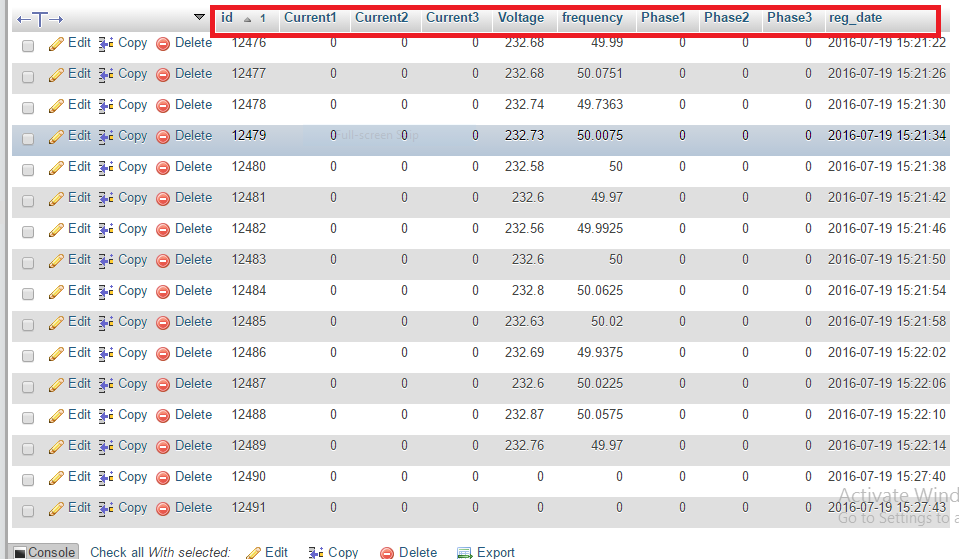
\includegraphics[width=15cm]{reading.png}
				\caption{Database table - $reading$}
				\label{1}
			\end{figure}
			
			\item{Table name - $para$, It only keeps the latest value under columns $RT$, infront of different row ids assigned to it. }
			
			\begin{figure}[H]
				\centering
				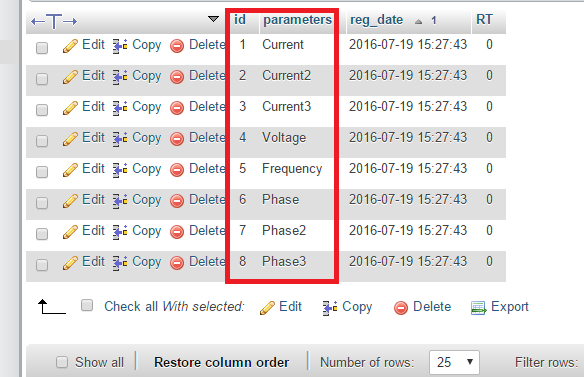
\includegraphics[width=15cm]{para.png}
				\caption{Database table - $para$}
				\label{2}
			\end{figure}
			
		\end{itemize}    
		\newpage	
	\end{itemize}
	\item{Real Time Plotting Graphs}
	\begin{itemize}
		\item{$current.html$ makes AJAX requests to $refresh.php$ which connects to database and updates it with latest data.}
		\item{With the latest data made available continuosly,Real Time updating graphs can be plotted.}
		\item{As the $chart.js$ will need data in JSON format, it requests to $action\_page.php$ to fulfill this requirement. }
	\end{itemize}
	\begin{figure}[H]
		\centering
		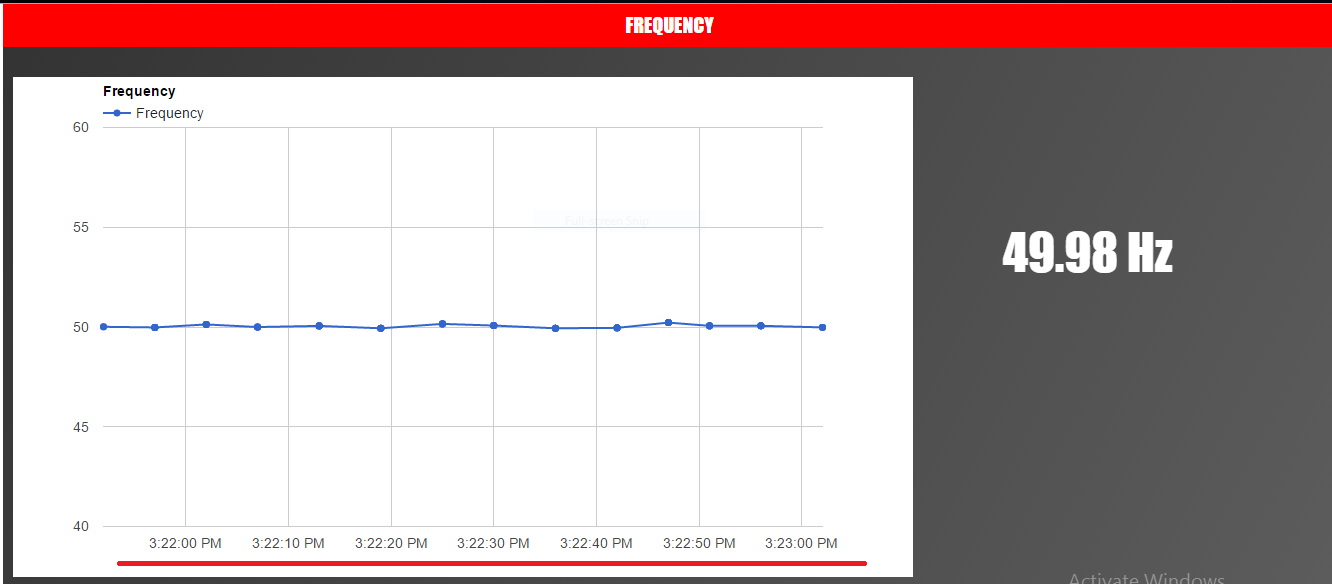
\includegraphics[width=15cm]{freq1.png} 
		\caption{Real Time Frequency plot at $3:22$ }
		\label{3}	
	\end{figure}
	
	\begin{figure}
		\centering
		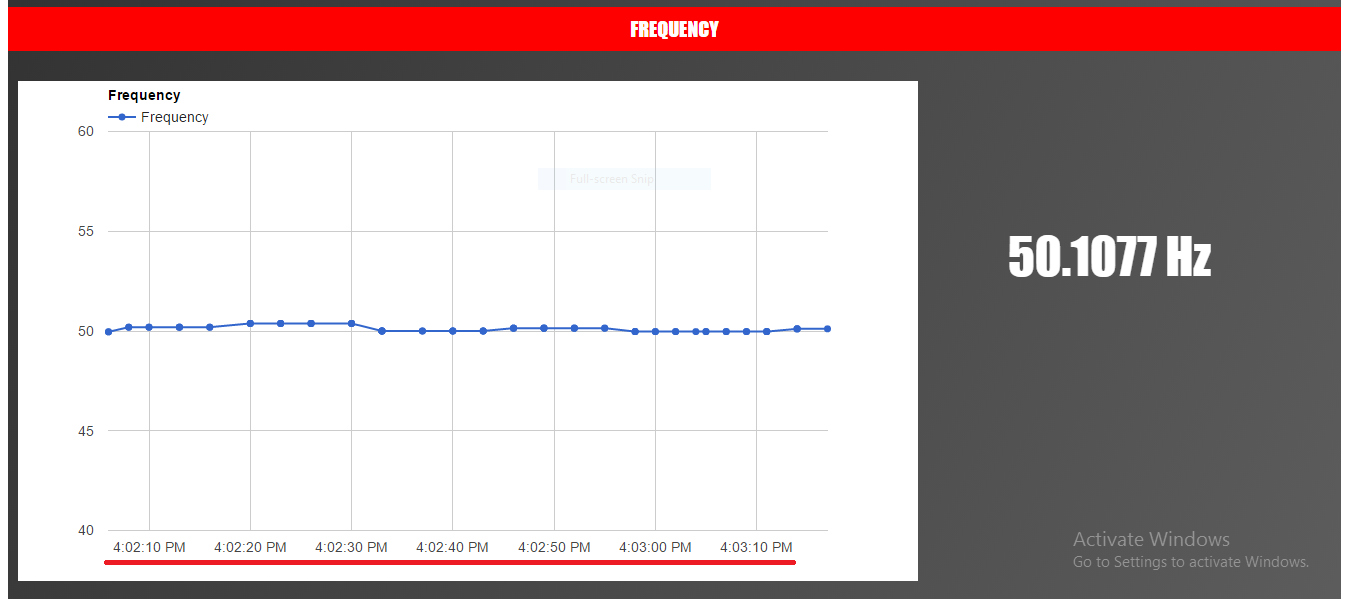
\includegraphics[width=15cm]{freq_mov.png}
		\caption{Real Time Frequency plot at $4:02$ }	
		\label{4}
	\end{figure}
	\newpage
	\item{Plotting the logged data }
	\begin{itemize}	
		\item{The logged data is gathered and and converted into JSON by $action\_graph\_week.php$}
		\begin{figure}
			\centering
			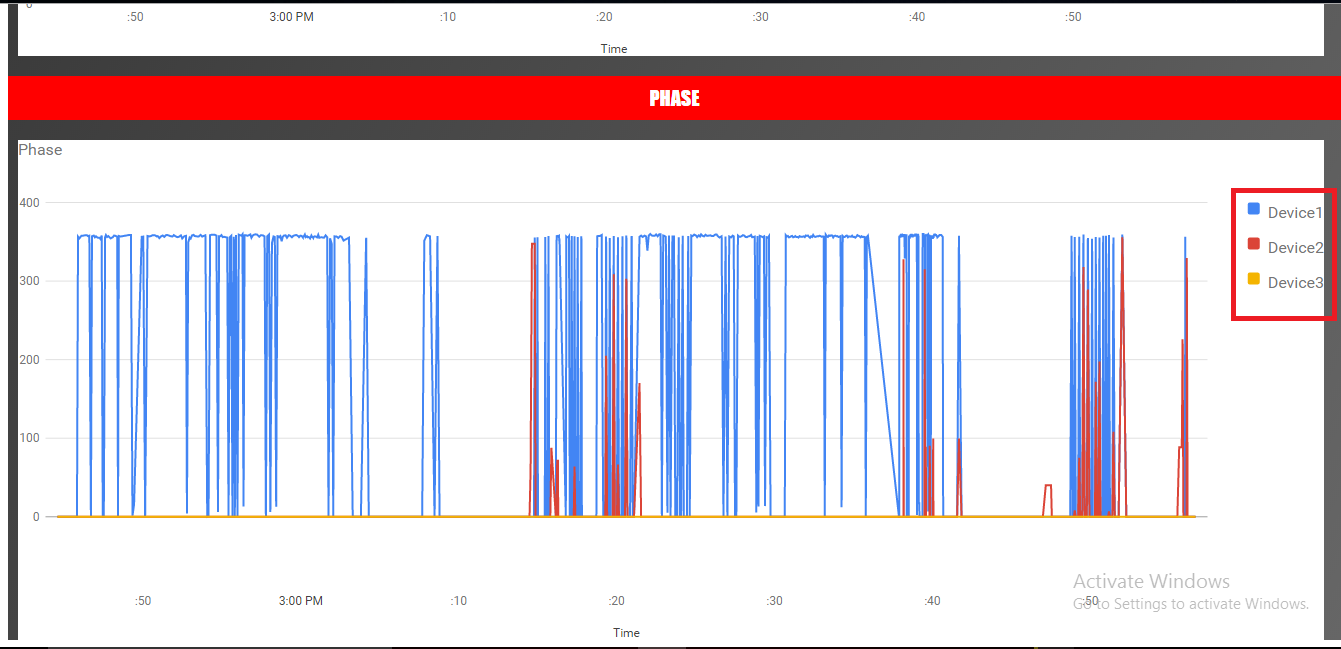
\includegraphics[width=15cm]{phase_today.png}
			\caption{Logged Phase data}
			\label{5}
		\end{figure}
		
		\begin{figure}
			\centering
			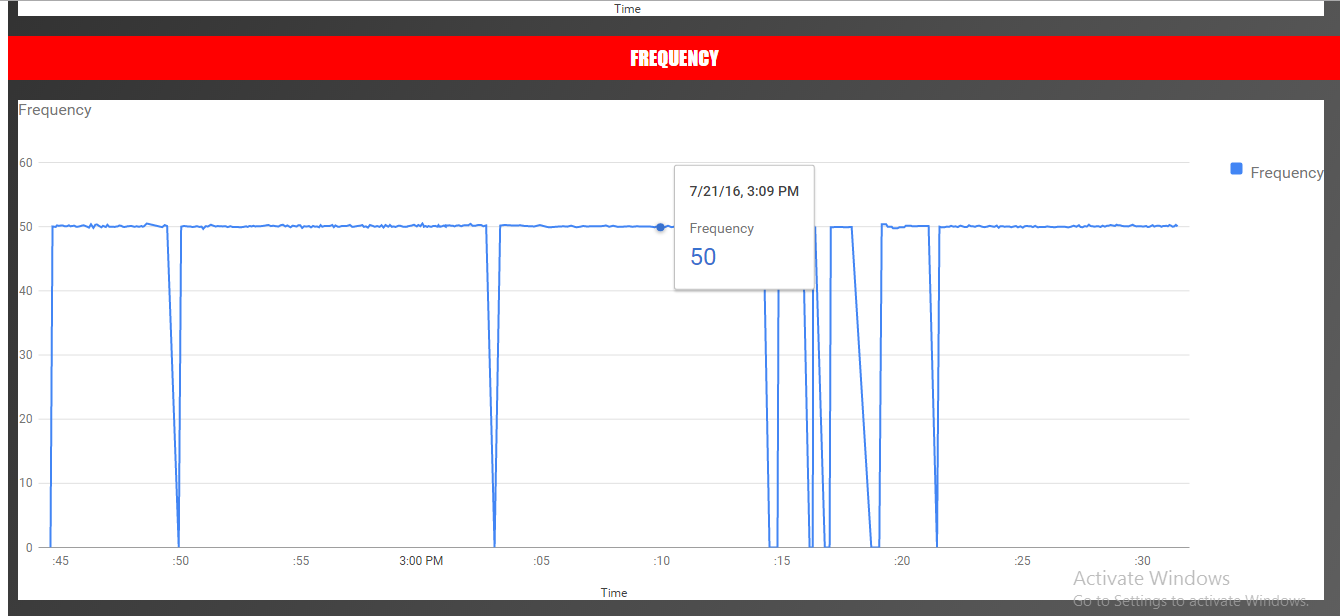
\includegraphics[width=15cm]{frequency_today.png}
			\caption{Logged Frequency Data}
			\label{6}
		\end{figure}
		
		
		
		\begin{figure}[H]  \centering
			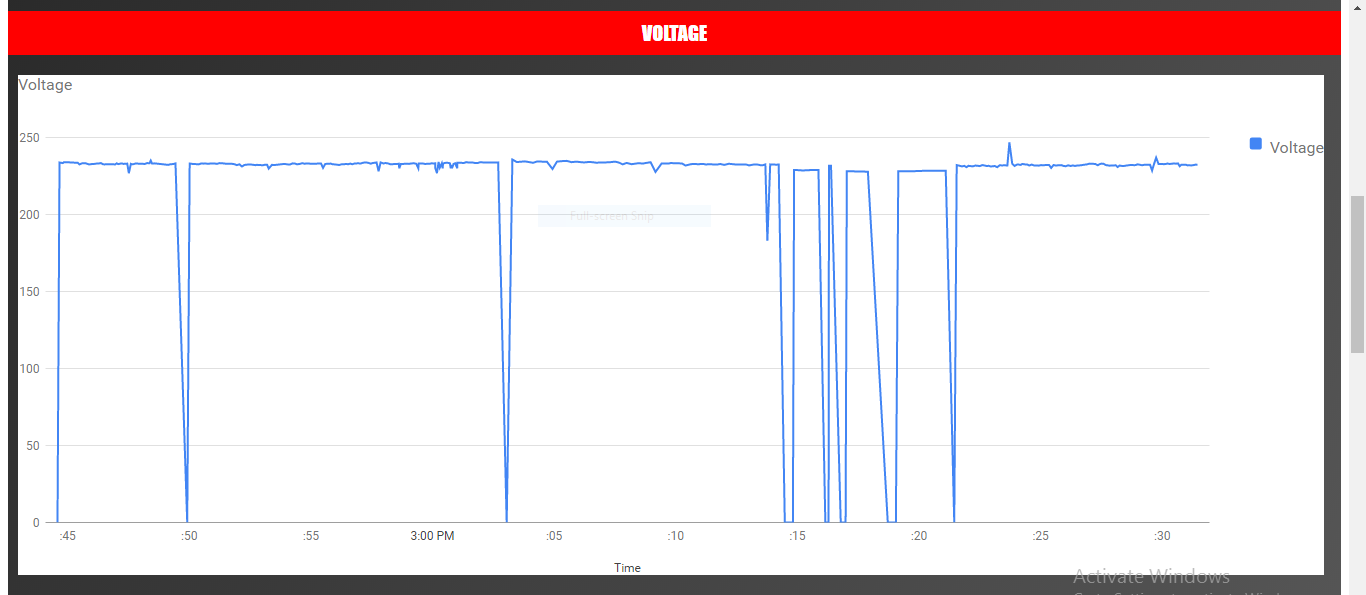
\includegraphics[width=14cm]{voltage_today.png}
			\caption{Logged Voltage Data}
			\label{7}
		\end{figure}
		
		
		
		\begin{figure}[H]  \centering
			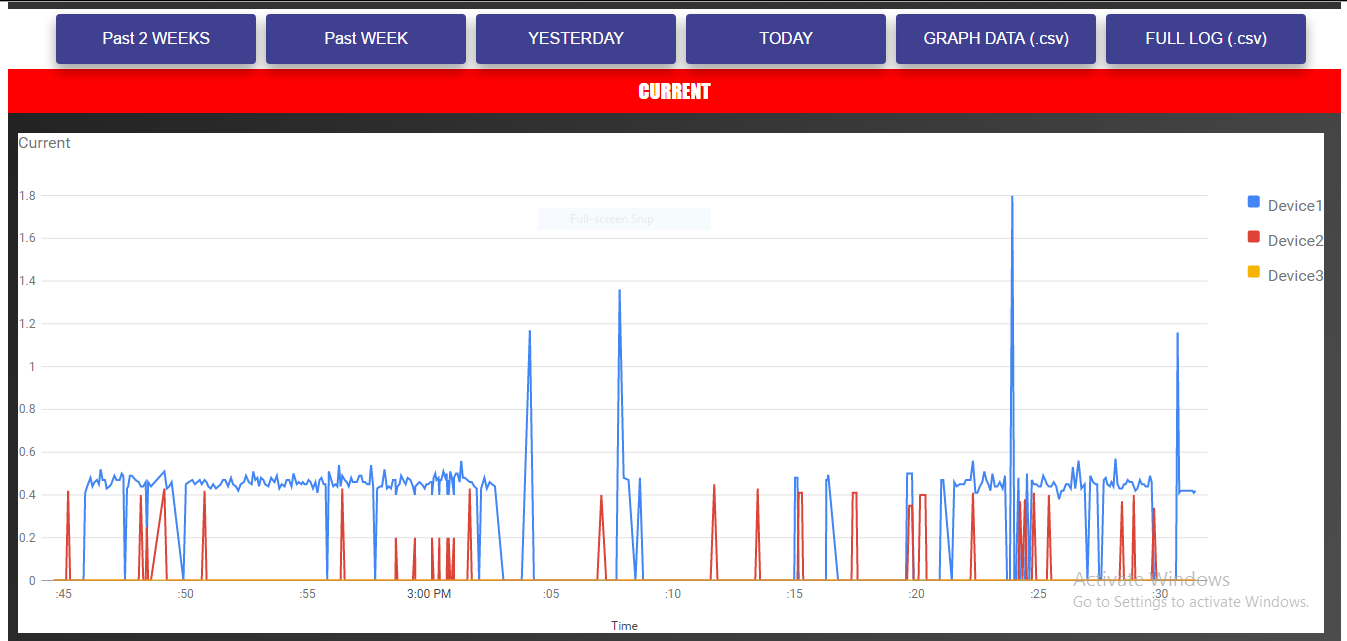
\includegraphics[width=15cm]{current_today.png}
			\caption{Logged Current Data}
			\label{8}
		\end{figure}
		
		
		
		\item{The graph is plotted by $stable\_chart\_loop.js$ which creates a graph according to datatable generated after user selected a particular period.}
		
		
		\begin{figure}[H]  \centering
			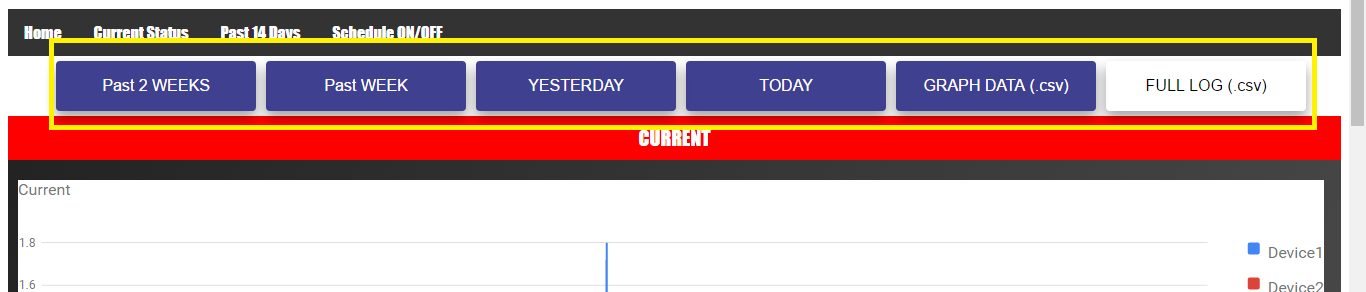
\includegraphics[width=15cm]{selection_buttons.png}
			\caption{Selection Buttons}
			\label{9}
		\end{figure}
		
		\item{As shown in above image, user can select the period ,which will then accordingly request and generate JSON data required for $stable\_chart\_loop.js$ }
		
		\item{The graph can be selectively highlighted and observed with timestamp and value on tool-tip.}
		
		\hspace{10px}
		
		\begin{figure}[H]  \centering
			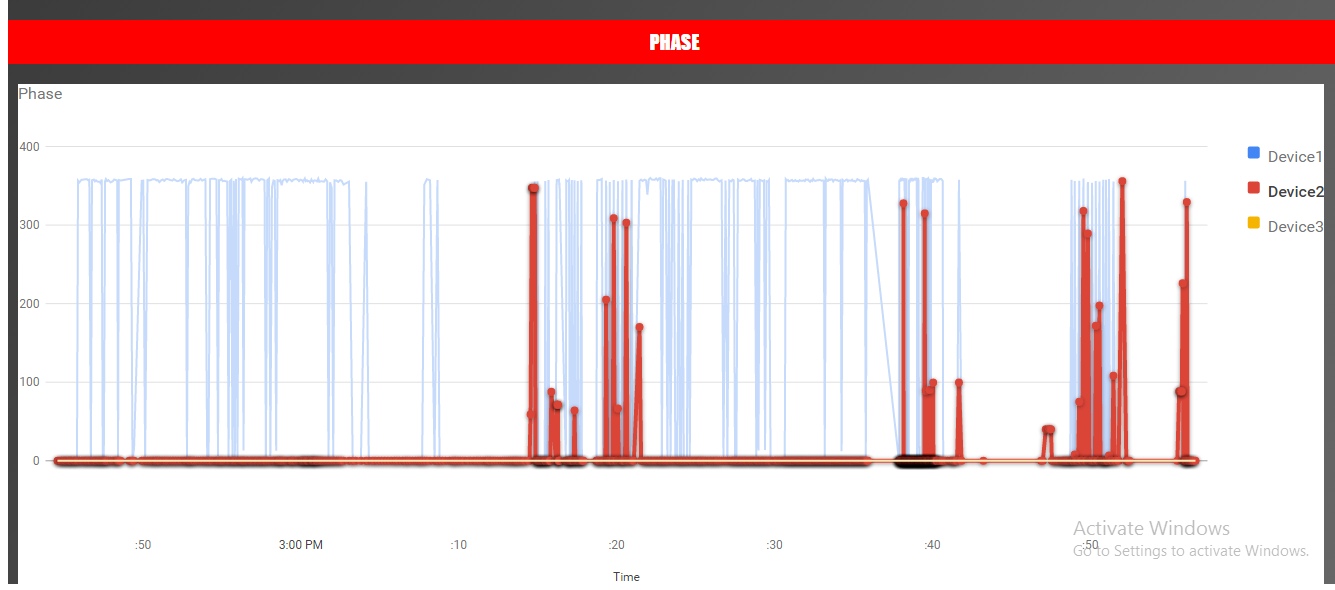
\includegraphics[width=15cm]{selectively_graph.png}
			\label{10}
			\caption{ Selective view of graphs for multiple devices.} 
		\end{figure}
		
		\hspace{10px}
		
	\end{itemize}
	\item{Feedback System. }
	\begin{itemize}	
		\item{In request cc3200 also provides feedback using $ds1,ds2,ds3$ }
		\item{In response server will update it with a boolean sequence for eg.$100,110,000...$ indicating switch status for each one of the 3 devices  } 
		\item{Then the server waits for feedback in next request, which are provided by cc3200 in variables $ds1,ds2,ds3$}
		
		
		\begin{figure}[H]  \centering
			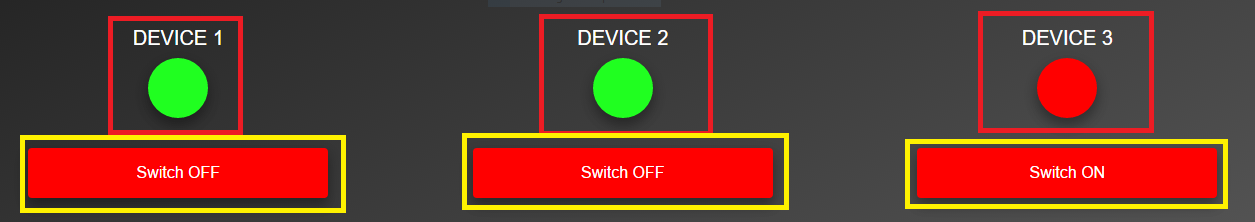
\includegraphics[width=15cm]{feedback.png}
			\label{11}
			\caption{Feedback system}
		\end{figure}
		\hspace{10px}
		\item{The above image shows circular blocks which shows current device status according to the board, obtained in request.\\ If  a device is showing OFF when it should be ON or showing ON when it should be off, then fallacy can be detected.It indicates that maybe there is no device or it is not functioning properly }
	\end{itemize}
	\item{Scheduling and Control}
	\begin{itemize}	
		\item{The scheduling page allows user to schedule ON and OFF (as Radio buttons)  and selection 'FROM' time and 'TO' time using input text field and datetimepicker.}
		\hspace{10px}
		
		\begin{figure}[H]  \centering
			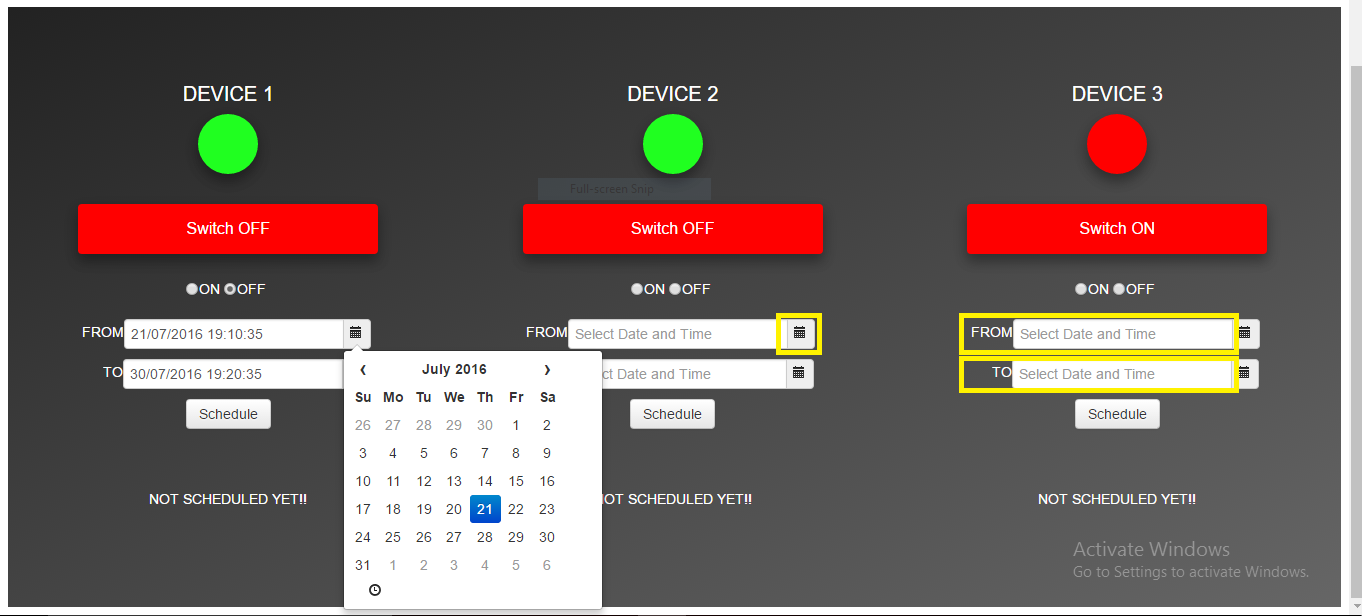
\includegraphics[width=15cm]{scheduler.png}
			\caption{ ON/OFF Scheduler}
			\label{17}
		\end{figure}
		
		\item{The Scheduling datetime is submitted to $selection.php$ which update values in database, which are then further compared with every timestamp and a boolean string response for conneced devices}
		
		\begin{figure}[H]  \centering
			\includegraphics[width=15cm]{scheduled.png}
			\caption{ Database Table $scheduled$ }
			\label{18}
		\end{figure}
		\item{Initial status of $button\_change$ is 1, which means scheduling is inactive.}
		\begin{figure}[H]  \centering
			\includegraphics[width=15cm]{scheduled_table.png}
			\caption{ Database Table updated values in table }
			\label{19}
		\end{figure}
		
		\item{Initial status of $button\_change$ is 0, with updated values of $Switch\_on$ time and $Switch\_off$ time(Scheduled values on left frame for reference).}
		
		\item{As $Switch_off$ Time is smaller than $Switch_on$ time, the Scheduler will automatically Switch OFF the device and wait for next Switch ON command.}
		
		\item{Buttons are available for all three devices, which have the capability to switch devices off/on.}
		
		
		\begin{figure}[H]  \centering
			\includegraphics[width=13cm]{power.png}
			\caption{ Database table $Power$}
			\label{20}
		\end{figure}
		
		\item{The button data is submitted to $button\_status.php$, $button\_status2.php$, $button\_status.php3$ with a value for variable $q$. which upadates the above shown table.}
		
	\end{itemize}
\end{itemize}	
\newpage
\section{Use and Demo}
\begin{itemize}
	\item{Configure the Smart Switch-board using terminal based GUI }
	
	\begin{figure}[H]  \centering
		\includegraphics[width=13cm]{coolterm2.jpg}
		\caption{ Coolterm - 2}
		\label{34}
		
		\includegraphics[width=13cm]{coolterm3.jpg}
		\caption{Coolterm - 3}
		\label{30}
	\end{figure}
	\begin{figure}[H]  \centering
		\includegraphics[width=13cm]{coolterm4.jpg}
		\caption{Coolterm - 4}
		\label{31}
	\end{figure}
	\begin{figure}[H]  \centering
		\includegraphics[width=13cm]{coolterm5.jpg}
		\caption{Coolterm - 5}
		\label{32}
	\end{figure}    	
	\begin{figure}[H]  \centering
		\includegraphics[width=13cm]{coolterm6.jpg}
		\caption{ Coolterm - 6}
		\label{33}
		
	\end{figure}
	
	\item{Open the webpage.}
	
	
	\begin{figure}[H]  \centering
		\includegraphics[width=15cm]{homephp.png}
		\caption{Home Page}
		\label{21}
	\end{figure}
	
	
	\item{This is the home page of the web based GUI, with 3 buttons redirecting buttons.}
	\item{ Under the title of page, a navigation bar is present.}
	
	\item{Next is the current status page.See \autoref{27}.\\ The first Division shows the current(in A) flowing in the 3 devices. \\BLUE for Device 1\\RED for device 2\\YELLOW for device 3 }
	
	\begin{figure}%
		\centering
		\subfloat[Live Data 1]{{\includegraphics[width=6cm]{Live_data} }}%
		\qquad
		\subfloat[Live Data 2]{{\includegraphics[width=6cm]{Live_data2} }}%
		\caption{Real time updating graph}%
		\label{27}%
	\end{figure}
	
	\item{Divisions for voltage(in V)and frequency(in Hz) follow Current's division.	
		\\ Only one line chart is being made for these two parameters as they are same for all three devices.}
	
	\item{Last division represents phase difference(in deg) of the three connected devices. See  \autoref{27} for reference .\\BLUE for device 1\\RED for device 2\\YELLOW for device 3 } 
	
	\begin{figure}[H]
		\centering
		\includegraphics[width=15cm]{logging_page.png}
		\caption{Logging page}
		\label{24}
	\end{figure}
	
	
	\item{\autoref{24} shows the logging page.}
	\item{As shown in the \autoref{9} the first four buttons provided are for period selection, and the last two are download links for .csv format for graph data and complete log data respectively.   }
	
	\item{By clicking any of the four buttons will plot the graph for the given period, and $Graph Data$ download link will generate a log for that specific period in .csv format.}
	
	\begin{figure}[H]  \centering
		\includegraphics[width=15cm]{log.png}
		\caption{Graph Data Log}
		\label{22}
	\end{figure}
	%*************************************************************************
	\item{$Today$ button will generate graph with Only That day's data.\\$Yesterday$ button will generate graph for previous data only.\\
		$Past\ week$ will generate filtered hourly data in the past week.\\
		$ Past\ 2\ Weeks$  will generate filtered hourly data in the past 2 weeks.\\ These are defined in $action\_graph\_week.php$.}
	
	
	%-------------------------------------------------------------------------- 
	
	\item{Full log in .csv format is always available for the user to download .}
	
	\begin{figure}[H]  \centering
		\includegraphics[width=15cm]{full.png}
		\caption{Full Log}
		\label{26}
	\end{figure}
	%***********************************************************************
	\item{ The last page is $Schedule\ ON/OFF$.See \autoref{17} .This is the controlling page with features like scheduling and switching ON/OFF.\\ The button highlighted in the image is the switch.\\It can be noted that tbhe text on it changes according to current button status.\\
		Above switch, there is a circular block which indicates the actual device status.\\
		GREEN represents ON status.\\RED represents OFF status. As depicted in figure 1.17.}	
	\item{Just below every switch button there is a scheduler which can schedule ON/OFF.\\
		The user first have to make a choice between ON/OFF radio buttons.If no selection is made it will be automatically counted as OFF . }
	\item{ Then the user have to fill the two input fields namely $FROM$ and $TO$ as per requirement.See \autoref{17}}
	\item{Scheduled Time-interval and Type will be notified as text.See \autoref{18}}
	
	%--------------------------------------------------------------------------
	
	
\end{itemize}

\section{Future Work}
\begin{itemize}
	\item{Current Web GUI is not responsive and will not work properly on mobile phones. Using Bootstrap (HTML,CSS framework) it can be done.}
	\item{Zoom Function can be added in charts for better user experience.}
	\item{Frequency feature can be added scheduling.}
	\item {Support for more devices can be added even when monitoring is available for few devices due to limited ADCs. }
	\item{Circuit can be miniaturized by using Redbear Wifi-mini aur cc3200 micro, which can increase portability}
	\item{Phase measurement accuracy can be improved.}
	
\end{itemize}
\newpage
\section{Bug report and Challenges}
\subsection*{Bug report}
\begin{itemize}
	\item For accurate measurement of phase please calculate the phase difference created by coupling capacitor applied to current wave for removing offset voltage.
	\item Use \textbf{TI-RTOS} \& \textbf{Free-RTOS} for fast processing and transient analysis of the electrical parameters.
	\item{SQL Injection }
	\item{HTTP communication protocol has been used.More secured protocols can be used.}
\end{itemize}
\subsection*{Challenges}
\begin{itemize}
	\item To add header files to the code composer studio project right click on project ,go to properties than select linked resources and than add $CC3200_skd$. After adding sdk to linked resources than again right click on project, go to GNU compiler and include directories to it.
	\item The debug mode of CCS load the program into RAM of CC3200 launchpad so to load program into ROM use \textbf{Uniflash}.
	\item Before loading the program into flash please follow the below procedure
	\begin{itemize}
		\item Format the whole CC3200 launchpad's ROM using \textbf{format} tab.
		\item Load \textbf{service pack}, which is compatible with your launchpad's version.
		\item Now load the .bin file of project. 
	\end{itemize} 
	\item For loading program into ROM select \textbf{mcu.bin} tab in Uniflash and than add the .bin file of the project.After adding the .bin file program MCU using program tab.
	\item To write program for CC3200-launchpad please take help from \textbf{Driverlib API's},\textbf{Simplelink API's} and all the API module files present inside CC3200sdk folder.
	   
\end{itemize}

\begin{thebibliography}{li}
		\item{Stack Overflow  \href{www.stackoverflow.com}{www.stackoverflow.com}}
		\item{TutorialsPoint  \href{tutorialspoint.com/}{www.tutorialspoint.com/}}
		\item{GitHub  \href{github.com}{www.github.com}}
		\item{W3Schools  \href{http://www.w3schools.com/}{www.w3schools.com/}}
		\item{TI E2E Community \href{TI E2E Community}{	https://e2e.ti.com/}}
		\item{Instructables \href{www.Instructables .com}{www.instructables .com}}
	
\end{thebibliography}


\chapter[Measurement board manual]{Measurement board manual}
\label{100}
\section{Abstract}
\hspace{7mm} The measurement board can process the input electrical signal and measure the basic electrical parameter from that. This is able to upload measured parameters to online Web servers.

\newpage
\section{Circuit diagram}
\begin{figure}[h]
	\includegraphics[width=380px,height=380px]{schematic}
\end{figure}
\newpage
\section{DIY}
Here we are including a special feature in the manual. By reading the manual now you can make this board by your self. To make it your self please follow the following instruction:
\subsection*{List of components}
\begin{tabular}{|l|c|c|}
	\hline
	\textbf{Name of component} & \textbf{Specification}& \textbf{Quantity}\\ \hline
	Resister& 10 ohm (1/4W)&1\\ \hline
	&330 ohm (1/4 W)&1 \\ \cline{2-3}
	&1K ohm (1/4W)&3 \\ \cline{2-3}
	&10K ohm (1/4W)&3 \\ \cline{2-3}
	&33K ohm (1/4W)&4 \\ \cline{2-3}
	&100K ohm (1/4W)&5 \\ \cline{2-3}
	&900K ohm (1/4W)&1 \\ \cline{2-3}
	&1M ohm (1/4W)&2 \\ \hline
	Electrostatic Capacitor& 0.1uF (50V)&1\\ \cline{2-3}
	&0.22uF (10V)&3 \\ \cline{2-3}
	&10uF (50V)&1 \\ \hline
	Ceramic capacitor& 0.01uF (103)&8 \\\hline
	Diode&IN4148 (high speed diode)&4 \\\hline
	Operational& LM324&2\\
	Amplifier&\textit{Quard opamp IC}&\\\hline
	Rectifier&DB-107&1 \\\hline
	Bug strip&Male(40x1)&2 \\\cline{2-3}
	&Female(40x1)&1\\\hline
	Breadboard \& Wires & -&1 \\\hline
	Soldering iron and wire& 40W&1 \\\hline
	General purpose PCB & 15cmx15cm&1 \\\hline	
\end{tabular}
\\\\\\\\
\subsection*{Procedure}
\begin{itemize}
	\item Before starting to building the circuit make sure you have gone through the circuit description. Because making circuit according to provided circuit doesn't make any sense.\\
	\newpage
	\item Buy all the component listed above it hardly cost you 500 rupees.\\
	\begin{center}
		\includegraphics[width=300px]{diy1}
	\end{center}
	
	\item First of check the circuit on the breadboard whether it is working or not, after checking the circuit on breadboard please connect your soldering Iron to plug and put up your PCB board on table.\\
	\begin{center}
		\includegraphics[width=300px]{diy2}
	\end{center}
	\item Start making small small circuit on different the part of PCB step by step as the circuit diagram is explained.
	\begin{center}
		\includegraphics[width=200px,angle=-90]{diy3}
	\end{center}
	\begin{center}
		\includegraphics[width=350px,angle=180]{diy4}
	\end{center}
	\item When small section of circuit schematic got completed on PCB than start connecting those small section according to label provided in schematic.
	\item Cheers!!! your measurement board is ready to use, now you can connect CC3200 launchpad to it and start software part. 
\end{itemize}
\section*{Pin Description}
\begin{center}
	\includegraphics[width=350px,height=400px]{board}
\end{center}
\begin{itemize}
	\item \textbf{PIN 1:} Hall sensor 1 input pin 
	\item \textbf{PIN 2:} Hall sensor 2 input pin
	\item \textbf{PIN 3:} Hall sensor 3 input pin
	\item \textbf{PIN 4:} DC blocked current signal 1
	\item \textbf{PIN 5:} DC blocked current signal 2
	\item \textbf{PIN 6:} DC blocked current signal 3
	\item \textbf{PIN 7 \& PIN 8:} Transformer(230V/9V) output pins
	\item \textbf{PIN 9:} processed voltage signal that will going into ADC pin
	\item \textbf{PIN 10:} processed current signal that will going into ADC pin
	\item \textbf{PIN 12:} Phase 1 signal 
	\item \textbf{PIN 14:} processed current signal that will going into ADC pin
	\item \textbf{PIN 15:} Phase 2 signal 
	\item \textbf{PIN 16:} processed current signal that will going into ADC pin
	\item \textbf{PIN 13:} Phase 3 signal 
	\item \textbf{PIN 17:} Frequency signal
	\item \textbf{PIN 18:} 5V header pins
	\item \textbf{PIN 19:} Vcc header pins
	\item \textbf{PIN 20:} Gnd header pins
	\item \textbf{PIN 21 \& PIN22:} Headers for mounting of CC3200 launchpad
\end{itemize}
\newpage
\section{Circuit output the each pin}
\subsection*{At Pin number 1,2 \& 3}
At these pins a current wave with 2.5V offset will appear.\\
	\begin{center}
		\textbf{OUT = $2.5 + asin(wt)$}
	\end{center}
	\begin{flushleft}
		\textbf{Where:}\\
			a = amplitude of $sin$ wave in V.\\
			$w$ = angular frequency of current signal in (rad/sec).\\
			t = time in sec.\\
	\end{flushleft}
	
\subsection*{At Pin number 4,5 \& 6}
At these pins a current wave without offset will appear.\\
\begin{center}
	\textbf{OUT = $asin(wt)$}
\end{center}
\begin{flushleft}
	\textbf{Where:}\\
	a = amplitude of $sin$ wave in V.\\
	$w$ = angular frequency of current signal in (rad/sec).\\
	t = time in sec.\\
\end{flushleft}

\subsection*{At Pin number 12,15,13 \& 17}
At these pins output of zero crossing circuit will appear.\\
\begin{center}
	\textbf{OUT = $5e^-^(^t^/^\tau^)$}
\end{center}
\begin{flushleft}
	\textbf{Where:}\\
	$\tau$ = time constant of zero crossing detector circuit.\\
	t = time in sec.\\
\end{flushleft}
\subsection*{At Pin number 9,10,14 \& 16}
Voltage and current signal manipulated according to reference voltage of CC3200 launchpad \\

\subsection*{At Pin number 18,19 \& 20}
5V, Vcc and ground pins on the measurement board.  \\
\subsection*{At Pin number 21 \& 22}
Headers for connecting CC3200-launchpad. \\

\end{document}

